\documentclass[10pt,twocolumn,letterpaper]{article}
% Venue-neutral preprint layout: 10pt, two columns, one-inch margins.
\usepackage[letterpaper,margin=1in]{geometry}
\setlength{\columnsep}{0.25in}
\usepackage{fontspec}
\setmainfont{TeX Gyre Termes}
\setsansfont[Scale=0.9]{TeX Gyre Heros}
\setmonofont[Scale=0.82]{Latin Modern Mono}
% Quoted fields keep every stored character: no TeX ligature substitutions.
\newfontfamily\fieldfont{TeX Gyre Heros}[Scale=0.88,RawFeature=-tlig]
% Math letters and digits are set in the text face so that symbols match the prose.
\DeclareSymbolFont{textitalic}{TU}{\rmdefault}{m}{it}
\DeclareSymbolFont{textroman}{TU}{\rmdefault}{m}{n}
\makeatletter
\@tfor\x:=ABCDEFGHIJKLMNOPQRSTUVWXYZabcdefghijklmnopqrstuvwxyz\do{%
  \expandafter\DeclareMathSymbol\expandafter{\x}{\mathalpha}{textitalic}{\expandafter`\x}}
\@tfor\x:=0123456789\do{%
  \expandafter\DeclareMathSymbol\expandafter{\x}{\mathalpha}{textroman}{\expandafter`\x}}
\makeatother
\usepackage{microtype,graphicx,booktabs,tabularx,longtable,array,amsmath,amssymb}
\usepackage{enumitem,caption,xcolor,xurl,needspace,float}
\usepackage[numbers,sort&compress]{natbib}
\usepackage[colorlinks=true,linkcolor=blue!35!black,citecolor=blue!35!black,urlcolor=blue!35!black]{hyperref}
\graphicspath{{assets/}}
\setlength{\emergencystretch}{2em}
\setlist{itemsep=1pt,topsep=3pt,leftmargin=1.4em}
\captionsetup{font=small,labelfont=bf,skip=5pt}
\newcolumntype{Y}{>{\raggedright\arraybackslash}X}
\newcolumntype{L}[1]{>{\raggedright\arraybackslash}p{#1}}
\newcolumntype{R}[1]{>{\raggedleft\arraybackslash}p{#1}}
\definecolor{meta}{HTML}{52514E}
\definecolor{rule}{HTML}{C9C8C2}

% Quotations. Text comes from sections/gen_quotes.tex, written by tools/06_quotes.py.
\makeatletter
\newcommand{\DeclareQuote}[2]{\expandafter\gdef\csname q@#1\endcsname{#2}}
\newcommand{\DeclareQuoteMeta}[2]{\expandafter\gdef\csname qm@#1\endcsname{#2}}
\newcommand{\Q}[1]{``{\fieldfont\csname q@#1\endcsname}''}
\newcommand{\QM}[1]{\csname qm@#1\endcsname}
\newcommand{\QB}[1]{\par\addvspace{3pt}\noindent\hspace{0.8em}\begin{minipage}{\dimexpr\linewidth-0.8em\relax}%
  \raggedright{\fieldfont\small \csname q@#1\endcsname}\par\vspace{1pt}{\footnotesize\color{meta}\csname qm@#1\endcsname}\end{minipage}\par\addvspace{4pt}}
% Table rows are read with the primitive so that a rule may follow them.
\newcommand{\rows}[1]{\@@input sections/#1.tex }
\makeatother
\newcommand{\incident}[2]{\par\addvspace{4pt}\noindent\textbf{Incident #1. #2}\ }
\newcommand{\src}[1]{{\footnotesize\color{meta}[#1]}}

% Appendix blocks for full stored fields.
\newcommand{\fieldhead}[2]{\par\addvspace{9pt}\Needspace{6\baselineskip}\noindent\textbf{#1.}\ {\small #2}\par}
\newcommand{\fieldtext}[2]{\par\addvspace{3pt}\noindent{\footnotesize\color{meta}#1}\par\nopagebreak
  \noindent\hspace{0.9em}\begin{minipage}[t]{\dimexpr\linewidth-0.9em\relax}\raggedright\fieldfont\small\setlength{\parskip}{3pt}#2\end{minipage}\par}
\newcommand{\fieldtextlong}[2]{\par\addvspace{3pt}\noindent{\footnotesize\color{meta}#1}\par\nopagebreak
  \begingroup\leftskip=0.9em\raggedright\fieldfont\small\setlength{\parskip}{3pt}\noindent #2\par\endgroup}
\newcommand{\fieldabsent}[2]{\par\addvspace{3pt}\noindent{\footnotesize\color{meta}#1.} {\small #2}\par}
\newcommand{\entry}[2]{G#1~d#2}

\hypersetup{pdftitle={What Can Be Raised? Financial Assessment and Economic Conduct of LLM Agents in Twenty Monopoly Games},pdfauthor={Kushagra Bharti}}
\title{\textbf{What Can Be Raised? Financial Assessment and\\Economic Conduct of LLM Agents in Twenty Monopoly Games}}
\author{Kushagra Bharti}
\date{Preprint, 14 November 2026}
\begin{document}
% Generated by tools/06_quotes.py from stored response fields. Do not edit by hand.
\DeclareQuote{g20-creditor}{p3's total liquidation value is \$1,414 (\$49 cash + \$675 from selling 9 Orange houses and 2 Brown hotels + \$690 from mortgaging 8 unmortgaged properties).}
\DeclareQuoteMeta{g20-creditor}{Gemini, authored note, G20 d325}
\DeclareQuote{g20-plan}{Full liquidation should yield \$1,414 including cash and all mortgages, enough for \$1,400 rent by \$14. Must sell all development and mortgage everything; survive rather than concede. If hotel sales leave four houses, sell those next evenly.}
\DeclareQuoteMeta{g20-plan}{Sol, authored note, G20 d327}
\DeclareQuote{g20-last}{Final \$30 mortgage covers \$16 shortfall, leaving \$14 after rent.}
\DeclareQuoteMeta{g20-last}{Sol, authored note, G20 d336}
\DeclareQuote{g13-select}{I owe \$750 and have \$168 cash (shortfall \$582). Since my non-Dark-Blue properties only mortgage for \$445 total, I must sell the house on Boardwalk (\$100) and mortgage Park Place (\$175) plus \$335 in non-Dark-Blue properties, keeping Boardwalk and Kentucky Avenue unmortgaged. Selling the house on Boardwalk first.}
\DeclareQuoteMeta{g13-select}{Gemini, authored note, G13 d195}
\DeclareQuote{g13-select-why}{I'm now leaning towards this approach to maximize my rental income potential.}
\DeclareQuoteMeta{g13-select-why}{Gemini, provider field, G13 d195}
\DeclareQuote{g5-revise}{I initially miscalculated! Selling the houses on Park Place and Boardwalk alone doesn't cover the debt. However, I can mortgage Park Place and Boardwalk after selling the houses!}
\DeclareQuoteMeta{g5-revise}{Gemini, provider field, G5 d263}
\DeclareQuote{g1-rule}{Must sell before yellows can be mortgaged.}
\DeclareQuoteMeta{g1-rule}{Grok, authored note, G1 d476}
\DeclareQuote{g18-rule}{which will allow me to mortgage St. Charles Place (\$70) on the next step}
\DeclareQuoteMeta{g18-rule}{Gemini, authored note, G18 d309}
\DeclareQuote{g2-opus-locked}{mortgaging the light-blue properties themselves for \$160 once the houses are gone}
\DeclareQuoteMeta{g2-opus-locked}{Opus, provider field, G2 d215}
\DeclareQuote{g15-max}{Max raise is \$520 (houses \$50 + Ill \$120 + Ventnor \$130 + Penn \$160 + Med \$30 + Baltic \$30). \$241+\$520=\$761 \textless{} \$800. Short \$39 even at full liquidation.}
\DeclareQuoteMeta{g15-max}{Grok, authored note, G15 d203}
\DeclareQuote{g10-sol-locked}{even subsequently mortgaging light blues adds only \$160}
\DeclareQuoteMeta{g10-sol-locked}{Sol, authored note, G10 d188}
\DeclareQuote{g12-false-note}{Three houses sell for \$225; Baltic and both light blues mortgage for \$130. With \$53 cash, maximum liquidity is \$408, below \$500 owed. No legal liquidation can save me.}
\DeclareQuoteMeta{g12-false-note}{Sol, authored note, G12 d190}
\DeclareQuote{g12-false-provider}{It seems like bankruptcy might transfer property anyway, so declaring insolvency could be the best option without needing further actions.}
\DeclareQuoteMeta{g12-false-provider}{Sol, provider field, G12 d190}
\DeclareQuote{g17-false-note}{I owe \$550 rent on Tennessee Avenue, and my total liquidatable value is only \$530 (5 Dark Blue houses at \$100 each plus \$30 for mortgaging Baltic Avenue). Since I cannot raise \$550, I must declare bankruptcy.}
\DeclareQuoteMeta{g17-false-note}{Gemini, authored note, G17 d234}
\DeclareQuote{g17-false-provider}{This won't cover my rent in full, so I will have to start thinking of additional options.}
\DeclareQuoteMeta{g17-false-provider}{Gemini, provider field, G17 d234}
\DeclareQuote{g3-listed}{Selling all twelve houses raises \$300 and mortgaging both railroads adds \$200: maximum \$914, insufficient.}
\DeclareQuoteMeta{g3-listed}{Sol, authored note, G3 d426}
\DeclareQuote{g5-listed}{Mortgaging my remaining properties and selling houses only gets me to 639 total}
\DeclareQuoteMeta{g5-listed}{Opus, provider field, G5 d309}
\DeclareQuote{g8-listed}{Only liquidation is 6 orange houses at \$50 = \$300, total \$386. No unmortgaged properties.}
\DeclareQuoteMeta{g8-listed}{Grok, authored note, G8 d280}
\DeclareQuote{g12-conflict-note2}{The sell\_houses call was the correct action. Declaring bankruptcy would be a mistake because staged even sales raise \$350 \textgreater{} \$207.}
\DeclareQuoteMeta{g12-conflict-note2}{Grok, authored note, G12 d249}
\DeclareQuote{g12-conflict-public}{Bankruptcy. The pinks go with the rest.}
\DeclareQuoteMeta{g12-conflict-public}{Grok, public message, G12 d249}
\DeclareQuote{g9-later}{I have already mortgaged Mediterranean Avenue and Pennsylvania Avenue. I will continue that strategy for consistency}
\DeclareQuoteMeta{g9-later}{Grok, provider field, G9 d196}
\DeclareQuote{g20-declare-note}{Selling first only hands the bank the house at half price before the same bankruptcy. Declare now.}
\DeclareQuoteMeta{g20-declare-note}{Grok, authored note, G20 d273}
\DeclareQuote{g19-rules-provider}{Under standard rules, a bankrupt player must turn over all assets to the creditor, and mortgaged properties transfer with their mortgage. The engine might enforce different rules.}
\DeclareQuoteMeta{g19-rules-provider}{Grok, provider field, G19 d224}
\DeclareQuote{g18-fee}{mortgaging it before declaring bankruptcy forces p4 to pay the 10\% mortgage transfer fee.}
\DeclareQuoteMeta{g18-fee}{Gemini, authored note, G18 d344}
\DeclareQuote{g18-inherit}{Must not go bankrupt — p1 would inherit built dark blues and I am eliminated.}
\DeclareQuoteMeta{g18-inherit}{Grok, authored note, G18 d313}
\DeclareQuote{g15-refusal-note}{Trade gives p4 Atlantic+Ventnor+Marvin and \textasciitilde{}\$830 plus mortgage capacity to drop 5+ yellow houses (\$150) immediately, then they roll again on doubles. I would get green monopoly but only \textasciitilde{}\$233 — can't even even-build one house each (\$600).}
\DeclareQuoteMeta{g15-refusal-note}{Grok, authored note, G15 d169}
\DeclareQuote{g15-final}{No. \$250 doesn't fix it. You'd still mortgage and drop houses on yellows before you roll again. Ventnor stays mine.}
\DeclareQuoteMeta{g15-final}{Grok, public message, G15 d175}
\DeclareQuote{g2-blocker-price}{\$450 is the price for the player who completes yellow. I'm not building it.}
\DeclareQuoteMeta{g2-blocker-price}{Grok, public message, G2 d120}
\DeclareQuote{g2-price}{Marvin completes your yellows. \$650 buys it; \$325 doesn't compensate for handing you that monopoly.}
\DeclareQuoteMeta{g2-price}{Sol, public message, G2 d124}
\DeclareQuote{g2-note}{At \$325 p4 retains \$520, enough for nine yellow houses immediately.}
\DeclareQuoteMeta{g2-note}{Sol, authored note, G2 d124}
\DeclareQuote{g7-public}{\$600, final.}
\DeclareQuoteMeta{g7-public}{Grok, public message, G7 d42}
\DeclareQuote{g7-private}{If they return at \$625, accept}
\DeclareQuoteMeta{g7-private}{Grok, authored note, G7 d42}
\DeclareQuote{g7-timed}{p4 just acquired the Dark Blue monopoly and spent down to \$84 building 3 houses. Since p4 now needs cash to add houses on Park Place and Boardwalk (\$200 each), they have strong incentive to sell New York Avenue for cash.}
\DeclareQuoteMeta{g7-timed}{Gemini, authored note, G7 d141}
\DeclareQuote{g13-pitch}{Opus — I'm on Atlantic with \$35. Next roll, 5/36 is Short Line and gpt inherits the yellows in bankruptcy. \$200 for the mortgaged Pennsylvania deed covers that rent. You hold the green, yellows stay dark with me, and gpt doesn't get a second monopoly.}
\DeclareQuoteMeta{g13-pitch}{Grok, public message, G13 d250}
\DeclareQuote{g13-floor}{\$130 only works if I also mortgage Ventnor and kills the only rent.}
\DeclareQuoteMeta{g13-floor}{Grok, authored note, G13 d252}
\DeclareQuote{g13-omit}{I will frame the \$130 offer as leaving me \$35 short of Short Line, omitting that I could mortgage Ventnor to survive.}
\DeclareQuoteMeta{g13-omit}{Grok, provider field, G13 d252}
\DeclareQuote{g13-buyer}{keeping grok solvent with cash from a \$200 purchase seems favorable overall — it's affordable, denies player 2 a monopoly, and the mortgage interest is minor.}
\DeclareQuoteMeta{g13-buyer}{Opus, provider field, G13 d253}
\DeclareQuote{g19-false}{Swap pinks plus \$150 your way. You already own St. James and New York — States is the third orange, not a pink closer. I take States so the pinks stay split; you keep the orange set and the cash.}
\DeclareQuoteMeta{g19-false}{Grok, public message, G19 d135}
\DeclareQuote{g19-abort}{Abort this trade. Do not send it.}
\DeclareQuoteMeta{g19-abort}{Grok, authored note, G19 d135}
\DeclareQuote{g19-correct}{States is pink, not orange—but Virginia plus \$150 works for me. Deal.}
\DeclareQuoteMeta{g19-correct}{Sol, public message, G19 d136}
\DeclareQuote{g20-appeal}{Ending my turn. Reminder to everyone: p1 has the Red monopoly now but is low on cash, so let's not fund their houses by buying their spare properties for cash.}
\DeclareQuoteMeta{g20-appeal}{Gemini, public message, G20 d96}
\DeclareQuote{g20-boycott}{p4 is organizing a cash boycott, so don't wait on a sale.}
\DeclareQuoteMeta{g20-boycott}{Grok, authored note, G20 d97}
\DeclareQuote{g20-refuse}{No thanks, p1. Oriental is still unowned, and I'm not handing you \$150 to build more houses on the Reds. Go ahead and mortgage it for \$50 if you need the cash.}
\DeclareQuoteMeta{g20-refuse}{Gemini, public message, G20 d101}
\DeclareQuote{g18-assure}{Thanks for the \$750. Your roll, p1. My Pacific offer still stands.}
\DeclareQuoteMeta{g18-assure}{Opus, public message, G18 d431}
\DeclareQuote{g18-reserve}{Buying Pacific might just prolong p1's survival, so maybe it's smarter to hold onto cash in case p1's orange hotels hit me with heavy rent.}
\DeclareQuoteMeta{g18-reserve}{Opus, provider field, G18 d431}
\DeclareQuote{g18-invoke}{I'll take your standing offer: Pacific for \$250.}
\DeclareQuoteMeta{g18-invoke}{Sol, public message, G18 d441}
\DeclareQuote{g18-withdraw}{That offer's off the table now. Things have changed. Your roll.}
\DeclareQuoteMeta{g18-withdraw}{Opus, public message, G18 d442}

\maketitle
\begin{abstract}
\noindent A player who cannot pay a debt must decide what its assets can raise. A player offered a trade must decide what the trade lets a rival raise and build. We study both judgments in twenty complete four-player Monopoly games among four configured LLM systems. The prompt states no rules and the financing menu lists deeds without prices. Agents paid 128 of the 131 payable debts among 188 that required financing. We show from the engine source that this outcome needed no route planning: under the recorded conditions any uninterrupted sequence of valid cash-raising actions pays. The informative records are the first choice to continue or stop, the text written with it, and the assets given up. Those first assessments are often exact. On unpayable debts, 43 of 48 state the full asset bound to the dollar. Of sixteen payable debts that need mortgages released by building sales, five responses state the dependency, three give an ordered route, five an inclusive budget and one raises it as a question. Two stop at the total the menu lists and declare bankruptcy. In bargaining, agents price a deed by what it lets the buyer build and finance a rival to keep an estate from a stronger creditor. The study is observational: one roster, five seeds, unequal response conditions, model-read text and no intervention.
\end{abstract}
\section{Introduction}

In one of the games we study, only two players remain. Gemini writes in its private note that Sol's holdings can raise \$1,414 if everything is sold and mortgaged, then builds a hotel that lifts one rent to \$1,400. Sol lands there with \$49. Its note reads \Q{g20-plan} Sol sells its buildings, mortgages eight deeds and pays. It has \$14 left. In another game Sol owes \$500, adds up \$408 and writes \Q{g12-false-note} It declares bankruptcy. Its holdings could have raised \$748.

Both responses answer one question: what can be raised? An agent that manages money must often value resources that are not on the screen in front of it, such as collateral that an earlier action must free or the cash a counterparty will hold after a sale. Monopoly makes such valuations checkable to the dollar, because the board fixes every mortgage and resale value and the engine records every state.

This paper asks what four configured LLM systems count as raisable money in twenty complete four-player games: their own when a debt arrives and a rival's when a trade is proposed. We check each count against board arithmetic and compare it with the action the engine applied. The populations are complete. They are all 188 debts that required financing and all 920 responses to trade offers.

\textbf{The environment does the route finding.} Agents paid 128 of 131 payable debts, including fourteen of sixteen that needed mortgages released by building sales. We show from the engine source and the recorded holdings that in all 131 entry states, any uninterrupted sequence of valid cash-raising actions pays (\S\ref{sec:task}). Payment therefore records that an agent did not stop. The informative records are the first choice to continue or stop, the text written with it, and the assets given up.

\textbf{First assessments are often exact.} The financing menu lists deeds without prices and the prompt states no rules. On unpayable debts, 43 of 48 first responses state the full asset bound, its proceeds or the remaining gap to the dollar. In the sixteen payable debts that need released collateral, five responses state the dependency, three give an ordered route, five give a budget that includes it and one raises it as a question (\S\ref{sec:texts}). Agents also choose what to give up. When listed mortgages were enough, they kept every building in 28 of 30 payments.

\textbf{The exceptions have a specific form.} Five first responses, from all four systems, stop at the total the first menu lists. Three concern debts that were unpayable either way. Two concern payable debts, and both agents declared. Of nine first actions that depart from the asset bound, six are Grok tool calls that contradict the action named in the same response, and one is a mortgage that Gemini justifies by a published settlement rule the engine does not implement (\S\ref{sec:stop}).

\textbf{Agents apply the same accounting to rivals.} In bargaining they price a deed by what it lets the buyer build, refuse their own monopoly because of the other side's budget, and finance a rival so that its estate does not pass to a stronger creditor (\S\ref{sec:bargain}). This evidence is exploratory.

The study is observational. It describes one roster under unequal response conditions, with no intervention, no executed reference policy and no human annotation. It does not rank models, identify why an assessment was incomplete, or measure whether a bargaining tactic worked. Appendix~\ref{app:scope} maps the project's original research questions to what this corpus does and does not establish.

\section{Games, agents and records}
\label{sec:setting}

\subsection{The games}
MonopolyBench~\cite{bharti2026monopolybench} runs four players on the standard forty-space board, each starting with \$1,500. Players buy or auction properties, trade through proposals and counters, build on complete color groups, and mortgage deeds. A game ends when one player remains, with no turn cap.

The roster is fixed: Sol (\path{openai/gpt-6.1-sol}), Gemini (\path{google/gemini-4-argon}), Opus (\path{anthropic/claude-opus-5.5}) and Grok (\path{x-ai/grok-4.7}), all called through OpenRouter at medium reasoning effort with no temperature or token limit set. Five seeds each receive four cyclic seat rotations, giving twenty games of 75 to 386 turns with 50,918 events, 6,989 decisions and 8,679 response attempts. Sol, Gemini, Opus and Grok win 8, 7, 3 and 2 games. Appendix~\ref{app:artifacts} lists seeds, source commits and game directories. Dollar amounts are game currency.

\subsection{What an agent is told}
The system prompt tells each agent to win, permits deception in public messages, and asks that private notes reflect true reasoning (Appendix~\ref{app:prompts}). It states no rules of play. Each request carries every player's cash, deeds, mortgages and buildings, the bank's building stock, twenty recent public events, and the agent's own ten most recent notes. Agents may choose only among actions the engine lists as legal.

When a player cannot pay a debt, the engine opens a financing menu. The menu names the deeds that can be mortgaged and the buildings that can be sold. It gives no dollar values. It carries one instruction: ``Choose exactly one liquidation action now. The engine will apply it, update your cash/assets, and ask you again if you still cannot pay. Declare bankruptcy only when you cannot or should not raise enough cash.'' The values and rules an agent writes down at this menu therefore come from what the model already knows, from its carried notes, or from earlier requests in the game.

\subsection{Published rules and implemented rules}
Table~\ref{tab:rules} compares the published rulebook~\cite{hasbroMonopolyRules} with the engine on the five rules that govern a debt. The rule that decides what can be raised is the same in both: a deed in a built group cannot be mortgaged until the group's buildings are sold. The rules that decide what stopping costs differ. The engine lets a player declare bankruptcy on a debt it could pay, passes buildings to a creditor intact, and charges nothing on inherited mortgages. Agents were told none of this. An agent that applies the rulebook is therefore right about what its assets can raise and can be wrong about what happens if it stops (\S\ref{sec:stop}).

\begin{table}[t]\centering\footnotesize
\begin{tabularx}{\linewidth}{@{}L{.20\linewidth}YY@{}}\toprule
Rule & Published rulebook & Engine in these games\\\midrule
Mortgaging in a built group & All buildings on the group must be sold first & Same\\
When bankruptcy occurs & When a player owes more than it can pay & Any financing menu, including on a payable debt\\
Buildings of a player bankrupt to another player & Sold to the bank at half price; creditor gets the cash & Pass to the creditor intact\\
Mortgaged deeds a creditor inherits & New owner pays 10\% interest at once & No charge\\
Selling hotels & All buildings on a group may be sold at once & A hotel becomes four houses, which the bank must have in stock\\\bottomrule
\end{tabularx}
\caption{Rules that govern a debt. The prompt states none of them. The financing menu shows the bankruptcy action and the currently legal mortgages and sales.}\label{tab:rules}
\end{table}

\subsection{Response channels and conditions}
The engine applies the tool call it receives. Four kinds of text can accompany that call. The \emph{authored note} is the private-thought argument of the applied call. The agent writes it, and the game returns it as memory in later requests. The \emph{public message} is another argument of the call and goes to all players. The \emph{provider reasoning field} is readable text that the gateway returns beside a response. The stored metadata labels it a reasoning summary for Sol and Grok and reasoning text for Gemini and Opus. No player receives it, and it can be summarized or end before a conclusion. \emph{Assistant content} is any other text returned with the call. The engine ignores it.

A note and the action it accompanies are parts of one response. The note is not a forecast taken before the action, and neither the order of fields nor the provider text shows which was computed first. A note can still come before what it describes in game time, as when it names collateral that no menu has yet offered.

Two response conditions matter. The provider refused 1,604 of Opus's first attempts, including every one in games 5 to 20, with a terms-of-service message about duplicating model outputs. The retry uses an action-only prompt that requests no note, and no retry was refused. Opus therefore has provider text but no authored note in most decisions. Grok ran with a required tool call while the others used automatic tool choice. In 139 Grok decisions the action named in its assistant content differs from the call received. Only Grok's content names actions, so this check can detect such a conflict for Grok alone, and the records do not show its cause.

\subsection{Measures}
A \emph{financing episode} begins at the first financing menu for a debt and ends at payment or elimination. At entry let $D$ be the debt, $C$ the cash, $S$ the resale value of all buildings, $M_0$ the mortgage value of the deeds the first menu lists, and $M_*$ the mortgage value of every unmortgaged deed. We use two sums:
\[U_0 = C + S + M_0,\qquad U_* = C + S + M_*.\]
$U_*$ is the \emph{full bound}. $U_0$ is the \emph{listed-only total}. It stops short of $U_*$ when buildings lock some deeds. A debt is \emph{payable} if the agent paid it or if a stored engine audit that predates this paper executed a legal payment sequence from the same state. A bound alone does not make a debt payable (\S\ref{sec:task}).

We read first responses in two ways. A number match asks whether a dollar figure equal to $U_*$ or $U_0$, or to the matching proceeds or gap, appears in the text. One LLM author also assigned each of sixteen focal responses to an evidence tier, with the supporting span printed in Appendix~\ref{app:coding}. Both readings have limits that we state once here. Neither is human annotation. A number match shows that a figure was written, not how the agent reached it. A provider field can be incomplete, so a resource missing from it may still have been considered. A total that includes a resource does not show knowledge of the rule that frees it. A stated dependency does not show that the statement produced the action.

\section{The financing task}
\label{sec:task}

\subsection{Every debt that required financing}
The twenty games contain 188 financing episodes. Agents paid 128 and were eliminated in sixty. The payments cover \$51,997 of debt through 180 mortgages and 89 building-sale calls. Sixty-seven took one action and sixty-one took two to ten. No first action and no payment came from the engine's fallback.

Three eliminations were declarations on debts that a stored audit shows were payable, so 131 debts were payable and agents paid 128. Fifty-six eliminations had $U_*<D$. One elimination, Opus in G7, shows why a bound is not a route. Its assets summed to \$1,310 against \$750 owed, but its only buildings were a hotel beside four-house lots and the bank held no houses, so the menu offered no sale. The published rules let all buildings on a group be sold at once (Table~\ref{tab:rules}). Opus wrote that its two listed mortgages would bring the total to \$440, took both, and the engine then closed the episode.

Table~\ref{tab:partition} divides the payable debts by what they required. The bound $U_0\ge D$ does not by itself prove that the middle group could be paid without released mortgages, since $S$ counts buildings the menu might not let a player sell. Here the evidence is direct. Forty-seven of the 53 were paid with no released mortgage. One has a stored sale-only payment sequence. The other five were paid with a released mortgage, and each also has a route without one that follows from its holdings and the bank's stock (Appendix~\ref{app:middle}).

\begin{table}[t]\centering\small
\begin{tabularx}{\linewidth}{@{}Yrr@{}}\toprule
What a payable debt required & Debts & Paid\\\midrule
Cash and listed mortgages ($C+M_0\ge D$) & 62 & 62\\
Building sales too; no released mortgage needed & 53 & 52\\
Mortgages released by sales ($U_0<D\le U_*$) & 16 & 14\\\midrule
All payable debts & 131 & 128\\\bottomrule
\end{tabularx}
\caption{The 131 payable debts. Payment establishes 128; a stored audit, not rerun here, executed legal payment sequences for the three declared.}\label{tab:partition}
\end{table}

\subsection{Continuing is enough to pay}
The engine pays a pending debt by itself as soon as cash covers it. If cash falls short and any mortgage or building sale is legal, it issues another menu. A mortgage never removes a sale option. A house sale never removes a mortgage option, and it returns a house to the bank.

Let $Q$ be cash plus the resale value of standing buildings plus the mortgage value of unmortgaged deeds. Every valid financing action leaves $Q$ unchanged and removes a building level or an unmortgaged deed, so a sequence of such actions is finite. If it ended unpaid with nothing left to sell or mortgage, cash would equal $Q$, which is at least the debt. The only other way to end unpaid is a state where assets remain but none is offered. That needs a hotel the bank cannot exchange.

We checked the 131 payable entry states against this. In all of them every built group is fully owned and evenly built. No hotel is present in 108. In twelve more, cash and listed mortgages already cover the debt. In nine more, the bank holds at least four houses per hotel. The last two hold one hotel in each of two groups, and a count of bank houses plus houses in hotel-free groups shows that a sale or an exchange always stays available (Appendix~\ref{app:proof}). So in every one of the 131 states, any uninterrupted sequence of valid cash-raising actions on the same debt ends in payment, provided the player never declares.

This is an argument from the frozen source and the recorded holdings. We ran no policy and report no baseline score. The argument does not cover invalid calls, call limits, provider failures or states outside these 131, and G7 shows that another state can strand its assets.

The argument changes what the outcomes mean. In these states payment follows from not stopping, so 128 payments do not show 128 planned routes, and a ten-action payment is not ten planning decisions. Three things remain free to vary: the first choice to continue or stop, what the agent says its assets can raise, and which assets it gives up.

\section{What the first responses count}
\label{sec:texts}

\subsection{Unpayable debts: the bound, to the dollar}
In 56 episodes the debt exceeds $U_*$. Eight of those menus offer bankruptcy alone. In the other 48 the agent could have financed or declared, and its first response usually says what its assets can raise. In 43 of the 48, the response contains the exact full bound, the exact proceeds $U_*-C$ or the exact gap $D-U_*$. Thirty of these figures are in authored notes and thirteen in provider fields. Grok's note in G15 is typical:
\QB{g15-max}
All four systems do this: Sol in 8 of 10 cases, Gemini in 11 of 11, Opus in 11 of 13 and Grok in 13 of 14. Two of the remaining five responses itemize every resource without a total. Three state the listed-only total (\S\ref{sec:false}).

\subsection{Payable debts that need released collateral}
Sixteen payable debts satisfy $U_0<D\le U_*$. Cash, every building and every listed mortgage together fall short, and the debt can be paid only with mortgages that a building sale releases. Agents paid fourteen. Figure~\ref{fig:sixteen} shows the sums and Appendix~\ref{app:texts} prints both text channels of all sixteen first responses in full.

\begin{figure*}[t]\centering
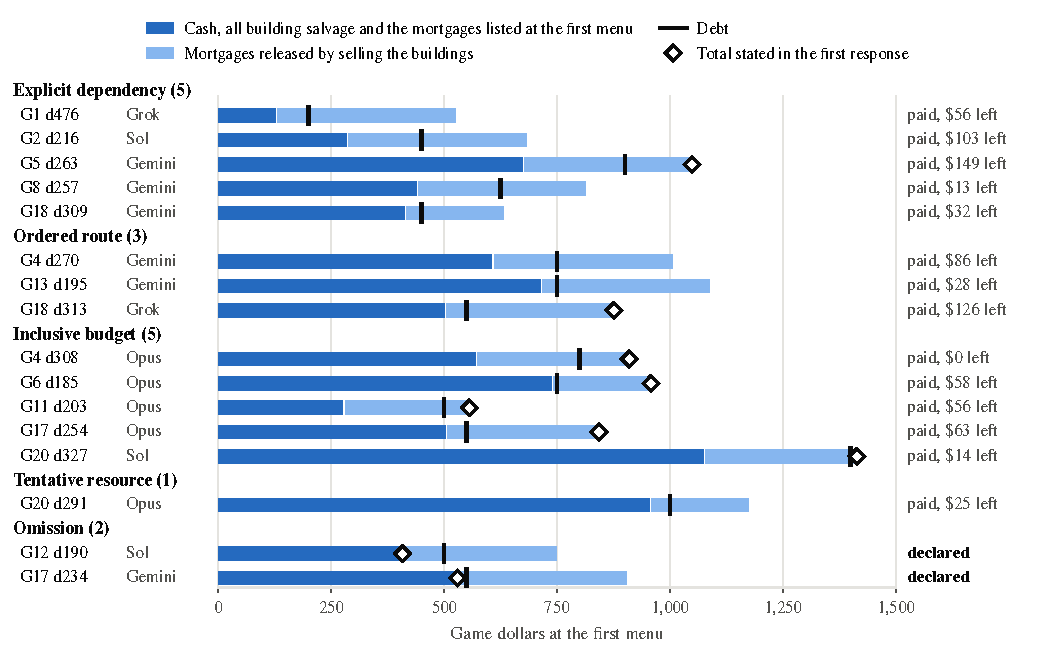
\includegraphics[width=.97\textwidth]{fig_sixteen.pdf}
\caption{The sixteen payable debts that required released collateral, grouped by how the first response treats that collateral. Every debt lies beyond the dark bar and within the pale one. A diamond marks a total stated in the response when it equals the listed-only total or the full bound (or the equivalent proceeds or remainder). Bars are resource sums, not liquidation plans.}\label{fig:sixteen}
\end{figure*}

The responses differ in how much they say about the dependency, and we sort them into five tiers (Table~\ref{tab:tiers}). Five state it. Grok writes \Q{g1-rule} Gemini writes that selling the houses \Q{g18-rule}. Three give an ordered route in which a sale precedes a named mortgage in the same group. Five give a budget that includes the locked deeds without saying what unlocks them. One raises the released mortgages as a question. Two leave them out.

\begin{table}[t]\centering\footnotesize
\begin{tabularx}{\linewidth}{@{}L{.25\linewidth}rY@{}}\toprule
Tier & $n$ & First responses\\\midrule
Explicit dependency & 5 & Grok G1; Sol G2; Gemini G5, G8, G18 d309\\
Ordered route & 3 & Gemini G4 d270, G13; Grok G18 d313\\
Inclusive budget & 5 & Opus G4 d308, G6, G11, G17 d254; Sol G20 d327\\
Tentative resource & 1 & Opus G20 d291\\
Omission & 2 & Sol G12 d190; Gemini G17 d234\\\bottomrule
\end{tabularx}
\caption{How sixteen first responses treat collateral that a sale must release. Tiers are one LLM author's reading of both channels, with evidence spans in Appendix~\ref{app:coding}.}\label{tab:tiers}
\end{table}

The tiers are not equally strong evidence. A statement or an ordered route shows that the response puts the sale first. An agent that summed every deed it owned would also write an inclusive budget. Four of the five inclusive budgets are Opus provider fields, the only channel Opus had, so tier and channel are confounded there.

The arithmetic is mostly right. In the authored notes and Opus's provider fields, every stated mortgage and resale value is correct except one: Sol gives the three yellow mortgages as \$430, and they total \$400. Seven successful responses contain a figure equal to the full bound, its proceeds or its remainder. Three state the cash that will remain, \$149, \$56 and \$14, and the route then leaves exactly that. Gemini's provider field in G5 shows an inventory being corrected inside one response:
\QB{g5-revise}

Errors and payment coexist. Sol's \$430 did not stop it paying. Opus in G20 d291 compares \$680 of proceeds with the whole \$1,000 debt and leaves out the \$275 it holds, so it calls itself \$725 short when the true gap is \$45. It then asks whether the pink deeds could be mortgaged once cleared, sells, and pays. In two of Gemini's successful responses the provider field ends before the released collateral appears, while the note in the same response states it. A provider field that stops early is therefore not evidence that the agent left a resource out.

\subsection{Two false budgets}
\label{sec:false}
Both failures among the sixteen are declarations at the first menu, and both follow a stated maximum:
\QB{g12-false-note}
\QB{g17-false-note}
Each sum is correct for what it counts, and each equals $U_0$ exactly. Sol leaves out \$340 of red mortgages and Gemini \$375 of dark-blue mortgages, the deeds their buildings stand on. The stored audit paid both debts from the same states with \$38 and \$180 to spare. Sol's provider field repeats the sum and continues \Q{g12-false-provider} Gemini's stops at \Q{g17-false-provider}

The same systems count the same kind of resource elsewhere. Sol pays two of its three debts in this group and Gemini five of six, one of them in G5 with the same two dark-blue deeds. The listed-only total is not confined to these two responses. Counting the sixteen payable debts and the 21 unpayable ones where buildings lock some deeds, 37 first responses face collateral that the menu does not list. Thirty-two count it or raise it. Five stop at the listed-only total: Sol twice, and Gemini, Opus and Grok once each. In three of the five the debt was unpayable either way, so the short count changed nothing. In the two payable cases it flipped the verdict.

The records do not say why these two inventories stopped where they did. Both agents carried earlier notes with the same reserve figures, \$130 and \$30. Those figures are also the true values of the listed mortgages, so the match cannot separate reuse of a note from a fresh count of the menu, and similar carried figures precede four payments in this group (Appendix~\ref{app:carried}). Counting what the menu lists, reusing an inventory written while the buildings were meant to stand, applying a known rule incompletely, and ordinary response variation all fit two cases. Sol's remark about property transfer shows that a declaration can also rest on more than the budget, and the prompt allows a player to stop when it ``cannot or should not'' raise the cash. The two budgets are false statements about what could be raised. Whether they were the whole reason for stopping is not identified.

\subsection{Choosing what to give up}
The engine stops asking once cash covers the debt, so the order of an agent's actions decides what it gives up. Sixty-two payments had enough cash and listed mortgages. The player held buildings in thirty of them, and in 28 it paid by mortgages alone and kept every building. In the 52 payments that needed sales but no released mortgage, 46 kept some buildings. Across all 128 payments, 122 left a deed unmortgaged, and in 119 the cash left over was smaller than the smallest house or mortgage given up, so no single unit in the route was surplus. We did not search for cheaper routes.

\incident{1}{A plan that names what to keep (G13).} Gemini owes \$750 with \$168. Its note sets the route:
\QB{g13-select}
The engine records one house sold, then Pacific, Electric Company, Indiana and Park Place mortgaged, for \$28 left. Boardwalk and Kentucky stay unmortgaged as planned. The bound here was \$1,088, so Gemini had \$338 of slack and chose which assets to spend. Its provider field gives the reason: \Q{g13-select-why}

\incident{2}{An exact budget on both sides of a debt (G20).} The note in Gemini's hotel build reads \Q{g20-creditor} Here p3 is Sol, and the two components are each \$25 off and cancel. Sol's note at the debt states the same \$1,414 and a \$14 remainder. At its tenth call the note reads \Q{g20-last} The debt sat \$14 below the bound, so full liquidation was the only end state that paid. The case shows two agents valuing nineteen assets to the dollar, not a choice among routes.

\section{Continuing or stopping}
\label{sec:stop}

Table~\ref{tab:first} sets the applied first action against the full bound for all 188 episodes. Agents start financing in 129 of the 132 episodes where the bound covers the debt. They declare at once in 50 of the 56 where it does not, and eight of those fifty menus offered nothing else.

\begin{table}[t]\centering\small
\begin{tabularx}{\linewidth}{@{}Yrrr@{}}\toprule
At the first menu & Episodes & Finance & Declare\\\midrule
Full bound covers the debt & 132 & 129 & 3\\
Full bound falls short & 56 & 6 & 50\\\bottomrule
\end{tabularx}
\caption{Applied first action in every financing episode. No first action is a fallback.}\label{tab:first}
\end{table}

We do not read this table as an accuracy score. The bound is not a feasibility label, as G7 shows. Eight declarations were forced. The prompt lets a player stop when it judges that it should not raise the cash, and a player may have reasons to finance a debt it cannot pay. The nine exceptions are more informative than the totals, and they fall into three kinds.

\textbf{Two false budgets.} Sol in G12 d190 and Gemini in G17 d234 declare on payable debts after stating the listed-only total (\S\ref{sec:false}).

\textbf{Six responses whose text and call disagree.} All six are Grok. In G12 d249 the debt was payable. Grok's assistant content names a house sale, and its note ends \Q{g12-conflict-note2} The call the engine received declares bankruptcy, and the public message in that call reads \Q{g12-conflict-public} In the other five, the debt exceeds the bound, the assistant content names bankruptcy and states a correct maximum, and the received call mortgages or sells. The notes inside those calls vary. Two say to declare, two claim that liquidation must come first, which the engine does not require, and one repeats a note from an earlier purchase. The note inside the sale call in G20 d273 reads \Q{g20-declare-note}

Across all 338 financing decisions, Grok's assistant content names an action 27 times and the received call differs in nine. No other system's content names an action in these decisions, so the check says nothing about them. These are disagreements between channels of one response. The engine applied a valid call, as its contract states, and the prose does not show what Grok would have chosen under another interface. For Table~\ref{tab:first} it matters that five of the six starts on unpayable debts carry text that favors stopping.

\textbf{One mortgage justified by a published rule.} Gemini in G18 d344 owes \$400, can raise \$382, and mortgages anyway. Its note says the mortgage will not cover the debt, but that \Q{g18-fee} Here p4 is Opus. The rulebook does charge the new owner of a mortgaged deed 10\% at once (Table~\ref{tab:rules}). This engine charges nothing. The belief matches the published rule and is wrong for this environment. Grok's provider field in G19 d224 states the uncertainty outright: \Q{g19-rules-provider}

Other responses reason about settlement in the engine's actual terms. Grok in G18 d313 refuses to stop because \Q{g18-inherit} Here p1 is Sol. That is what the engine does and what the rulebook does not. Agents bring rule knowledge to the stop decision, sometimes the rulebook's and sometimes the engine's, and the prompt gives them neither. Stop decisions in this corpus therefore mix a judgment about what can be raised with beliefs about what the creditor will receive. Only the first has an exact answer in the records.

\section{Counting a rival's money}
\label{sec:bargain}

A trade changes what the other player can raise and build. This section reports how agents respond to offers and what their texts say about a counterparty's finances. No reference value exists for a trade in a four-player game, so nothing here measures whether a response was good.

\subsection{All 920 responses}
The games contain 526 negotiation threads and 920 responses to offers: 113 acceptances, 394 counters and 413 rejections. Sol and Opus mostly counter (140 of 235 and 141 of 189 responses). Gemini and Grok mostly reject (180 of 242 and 149 of 254). Each accepts between 26 and 30 offers.

Table~\ref{tab:opening} gives every opening offer by form and by whose color group the trade would complete. Opening swaps that complete only the proposer's group are rejected 95 times in 116. Swaps that complete neither side's group are rejected 37 times in 72, a difference of 30.5 percentage points.

\begin{table*}[t]\centering\small
\begin{tabular}{@{}lrrrr@{}}\toprule
Trade would newly complete a group for & Swap & Cash bid & Cash ask & Other\\\midrule
\rows{gen_opening_rows}
\bottomrule
\end{tabular}
\caption{Every opening offer where acceptance was legal: $N$ [accepted/countered/rejected]. A swap moves deeds both ways, a cash bid asks for deeds and a cash ask offers them.}\label{tab:opening}
\end{table*}

The difference depends on who proposed. Grok wrote 36 of the 72 neither-completing swaps and fifteen of their seventeen acceptances, and thirteen of those fifteen offers came from calls whose assistant content named a different action. Without Grok-authored offers the rejection counts are 90 of 108 and 24 of 36, a difference of 16.7 points. Resampling the five seed blocks gives a percentile range of $-3.8$ to $31.9$ points for that figure. The range rests on five blocks and a contrast chosen after the fact. It shows instability and does not show that the association is absent. Opening cash bids differ by $-5.0$ points when pooled and by $-0.2$ to $+8.5$ points within recipients. Proposer-completing swaps are rejected more often in this cohort, and the size of the gap follows the mix of proposers. The data do not identify an effect of completion (Appendix~\ref{app:bargain}).

A separate population bears on what refusals say. Seventy-four rejections concern offers that would have completed the recipient's own group. Two model readings made for an earlier version of this study agree that 61 of the 74 texts cite a consequence for the rival. We did not repeat that reading and no person has checked it. These are different offers from the swap contrast, so the reading cannot explain it.

\subsection{Four incidents}
The system prompt permits deception in public messages, so no conduct below breaks an instruction. We selected the incidents for clarity. They show neither how often a tactic occurs nor whether it works. Three more are in Appendix~\ref{app:incidents}.

\incident{3}{Refusing one's own monopoly (G15).} Sol offers both its greens for Grok's Ventnor and \$100, which would complete a group for each. Grok holds \$333 and Sol \$730. Grok refuses, and its note counts both budgets (p4 is Sol):
\QB{g15-refusal-note}
The arithmetic is right. Sol would hold \$830 and Grok \$233, and a first even layer of green houses costs \$600. Sol raises the offer to both greens, Kentucky and \$250, and says this leaves Grok \$583 against its own \$480. Grok answers \Q{g15-final} Eighteen turns later Grok is eliminated and its deeds pass to Gemini. The refusal is argued from the rival's building budget. Whether it helped Grok is unknown.

\incident{4}{One deed, two prices (G2).} Grok owns no yellow deed and bids \$200 for Sol's Marvin Gardens to keep it from Opus. Sol asks \$450 and Grok objects \Q{g2-blocker-price} Opus, who owns the other two yellows and \$845, then bids \$325. Sol asks \$650:
\QB{g2-price}
Sol's note explains the price with a figure that is wrong, where p4 is Opus: \Q{g2-note} A yellow house costs \$150, so \$520 buys three. The pricing rule is clear and the rival's budget is overstated threefold. Opus calls \$450 final in public while its note sets a ceiling of about \$475. Sol keeps the deed.

\incident{5}{A bid timed to the seller's cash (G7).} Sol buys Park Place, builds three houses and has \$84 left. Gemini's note sees an opening (p4 is Sol):
\QB{g7-timed}
Gemini bids \$350 for New York Avenue, raises to \$520, and tells Sol the sum would give it exactly the \$600 that three more houses cost. Sol holds at \$700 and tells Gemini it can mortgage its other deeds to fund building. Gemini pays \$700, mortgages five deeds and builds four orange houses in the same turn. Each side computed the other's building budget. Earlier in that game Grok told Sol \Q{g7-public} while its note read \Q{g7-private}. Sol took \$600.

\incident{6}{Financing a rival to keep an estate from a creditor (G13).} Grok has \$35 and could owe Sol a \$200 rent on its next roll. It offers Opus a mortgaged deed for \$200, calling Sol ``gpt'':
\QB{g13-pitch}
Opus counters at \$130. Grok's note works out that \Q{g13-floor} Its provider field adds \Q{g13-omit} Opus holds \$1,926 and pays the \$200. Its provider field says that \Q{g13-buyer} Player 2 is Sol. The buyer paid to keep a third player from inheriting a color group. The seller's arithmetic was correct, and it left one financing option out of the pitch. Grok was eliminated on a \$200 debt to Sol 43 turns later.

\section{Related work}
\label{sec:related}

\textbf{Reachability and false impossibility.} Whether an action can become applicable after other actions is an established evaluation target. ACPBench includes an action-reachability task over planning domains, posed as single-turn questions~\cite{kokel2025acpbench}, and ACPBench Hard adds generative versions with validators~\cite{kokel2026acpbenchhard}. Models that wrongly call a solvable problem unsolvable are documented too: an evaluation of a reasoning model on PlanBench~\cite{valmeekam2023planbench} reports such claims on 11.5\% of solvable instances in one obfuscated domain~\cite{valmeekam2024lrm}. Our two false budgets are instances of a known kind of error. The records add its form in a natural setting: a correct sum over the resources the menu lists, written by an agent about its own assets and followed by an irreversible action.

\textbf{Plans, interactive action and menus.} ReAct interleaves reasoning, action and feedback~\cite{yao2023react}, and AutoPlanBench compares writing a whole plan with choosing one action at a time~\cite{stein2025autoplanbench}. Our financing task is interactive, and \S\ref{sec:task} shows that the interaction is enough to reach payment, so we do not treat payment as evidence of planning. Tool presentation also affects agents. One study holds a set of candidate tools fixed, changes only their order, and finds a change in task success~\cite{yan2026menu}. Our menus list only currently legal actions, but we varied nothing and cannot say whether another menu would change an assessment.

\textbf{Rules agents know.} Counterfactual variants of familiar tasks separate recall from reasoning~\cite{wu2024reciting}. Our release rule is the published one, so correct use of it does not show reasoning about an unfamiliar system. On settlement the environment departs from the rulebook without saying so, and some responses apply the rulebook.

\textbf{Text and action.} A model's explanation need not reflect what drove its output~\cite{turpin2023unfaithful,lanham2023faithfulness}, so we treat notes and provider fields as recorded statements. Agents that declare a planning structure often do not keep to it~\cite{oota2026declare}, and a workshop study of rule-altered chess describes an agent that reasons a move is illegal and submits it anyway~\cite{co2026atomic}. Grok's conflicts belong with these reports, though ours come from comparing response channels after the fact.

\textbf{Memory.} Agents follow retrieved experience, and errors in stored experience propagate~\cite{xiong2026memory}. We record what notes the two failing agents carried and find the evidence compatible with several accounts (\S\ref{sec:false}).

\textbf{Economic games.} AgentMonopoly studies model and persona effects across Monopoly games in which a player is eliminated when its cash goes negative, so no financing phase arises~\cite{wu2026agentmonopoly}. FinBoardBench includes Monopoly among three financial games, and its rules require a player short of cash to mortgage or sell houses~\cite{hu2026finboardbench}. Multi-step financing is therefore not new here, and that paper reports no analysis of the phase. We could not determine whether it permits bankruptcy on a payable debt, the condition that makes a premature stop observable in our games. A study of the multi-agent variant of Vending-Bench~\cite{backlund2025vendingbench} classifies every inter-agent email~\cite{li2026arena}, a population treatment of communication that our selected incidents do not attempt.

\textbf{Negotiation.} Earlier negotiation agents were evaluated on tasks with explicit private utilities~\cite{lewis2017deal,he2018decoupling}, and NegotiationArena studies LLM tactics in defined scenarios~\cite{bianchi2024negotiationarena}. In a full game an offer's value depends on later play, so we report responses without scoring them. Trade embargoes were simulated in Settlers of Catan with recipients that always comply, so those results concern an embargo that is obeyed~\cite{guhe2014persuasion}. Models of sales with identity-dependent externalities explain why the buyer's identity matters to third parties~\cite{jehiel1996externalities}. Incidents 4 and 6 show that concern. We do not test the theory.

\section{Scope and limitations}
\label{sec:limits}

\textbf{Design.} Twenty games are five seeds with four seat rotations of one roster. No seed and rotation pair was repeated, and each state was reached once. The games cannot separate a system from its seat, its opponents or its luck. Per-system counts describe what each system encountered: Opus faced 58 financing episodes and Grok 38. We make no ranking.

\textbf{Text.} The tier labels and the 61-of-74 reading are model readings without human validation. Number matches are exact but see only figures that were written. Opus's text comes from a different channel than the others' because of the refusal condition, and Grok's applied calls sometimes disagree with its content. Every statement about what an agent wrote should be read with its channel.

\textbf{Mechanism.} We ran no intervention on prompt, menu, rules, memory or response handling. The corpus does not identify why two inventories stopped at the listed-only total, whether a written assessment shaped the action or followed it, or what causes Grok's channel conflicts.

\textbf{Reference points.} The continued-financing result is an argument from source, not a measured baseline. Three payment witnesses and one menu search come from an earlier engine audit that we did not rerun. We computed no least-cost liquidation and no trade values, so nothing here is a statement about optimal play.

\textbf{Selection.} The necessary-collateral partition, the bargaining contrast and the incidents were chosen after looking at the games.

\section{Conclusion}

When a debt arrived, these agents usually wrote down what their assets could raise, and the figure was usually right to the dollar, with no price list and no rules in the prompt. Their first actions mostly followed the asset bound, and six of the nine departures were one system's calls contradicting its own text. Continuing to finance was enough to pay every payable debt, so the informative behavior lies in the first assessments and in the choice of what to give up. The same accounting appears in bargaining, where agents argue from a rival's building budget and from who would inherit an estate. Why a count stopped short, and whether a tactic paid, need a different design.

\label{mainend}
\begingroup\small\setlength{\bibsep}{2pt}
\bibliographystyle{plainnat}\bibliography{references}
\endgroup
\clearpage\onecolumn\appendix
\section{What the corpus supports for each original question}
\label{app:scope}
The project began with eight research questions and three cross-cutting ones. Table~\ref{tab:scope} states, for each, what these twenty games establish and what they leave open. An open entry means the design cannot measure the construct. It is not evidence that an ability is absent.

\begin{longtable}{@{}L{.20\linewidth}L{.40\linewidth}L{.34\linewidth}@{}}
\caption{Supported scope for the eight questions and for A to C.}\label{tab:scope}\\
\toprule Question & Established in this corpus & Not established\\\midrule\endfirsthead
\toprule Question & Established in this corpus & Not established\\\midrule\endhead
1. Strategic reasoning & Refusals and prices argued from a rival's building budget; first financing actions set against the asset bound for all 188 episodes, with the nine departures decomposed & Optimal play, regret, or a strategic score\\
2. Opponent modeling & Stated figures for a counterparty's cash, costs and liquidation value, some exact (G20) and some wrong (G2) & Calibration of beliefs; transfer to unfamiliar opponents\\
3. Negotiation and deception & All 920 responses by form and completion; two countering and two rejecting response styles; a permitted bluff, an omission, a correction, an appeal and a withdrawn assurance & Whether any tactic persuaded; prevalence of deception; welfare or fairness\\
4. Planning and memory & Stated dependencies and ordered routes before the menu offers the resource; a named selection of assets carried out exactly (G13); what notes each agent carried & A general planning ability; any benefit or harm from memory\\
5. Adaptation and learning & An inventory revised inside one response (G5); offers revised within threads & Learning from feedback across games or turns\\
6. Economic judgment and risk & Exact asset bounds in 43 of 48 unpayable first assessments; five listed-only totals; mortgage-first financing that kept buildings in 28 of 30 cases & Least-cost liquidation, reserve policy, or risk-adjusted value\\
7. Collective behavior & One public appeal to deny a rival cash, with the speaker's own refusal and another player's contrary offer & A coalition, collusion, or its effects\\
8. Evaluation validity & That payment here follows from not stopping; undisclosed differences between published and implemented rules; unequal channels across systems & Performance under a corrected interface or disclosed rules\\\midrule
A. Strategic language versus action & Agreement between first action and asset bound; six Grok responses whose text and call disagree; two false budgets acted on & A causal relation between a written assessment and the action\\
B. General versus multi-agent ability & Nothing. The roster has four unequal configurations and no external capability measure was matched to them & Any relation between general ability and play\\
C. Skill versus luck & Wins by system (8, 7, 3, 2) and by seat (7, 7, 3, 3) & Shares of skill, seat and luck in winning\\\bottomrule
\end{longtable}

\section{Why continued financing pays}
\label{app:proof}
This appendix gives the argument of \S\ref{sec:task} in full. It reads the engine source at the two commits used for the games, which are identical for the files involved, and the holdings recorded at the first menu of each payable debt. No policy, engine step, replay or search was run.

\textbf{Claim.} In each of the 131 payable entry states, every uninterrupted sequence of valid financing actions that each raise cash ends with the current debt paid, provided the player does not declare bankruptcy.

\textbf{What the claim excludes.} Invalid calls, empty sale plans, limits on calls or time, provider failures, a later debt in the same payment queue, and any state outside the 131. It is not a statement that an arbitrary agent would pay, and it says nothing about cost.

\textbf{Source facts.} File \path{python/packages/engine/src/monopoly_engine/engine.py}.
\begin{enumerate}
\item \path{_resolve_pending_payment}: after each financing action, if cash covers the amount the engine pays. Otherwise it computes the available mortgages and sales. If neither list has an entry it ends the episode in bankruptcy. If either has an entry it issues another financing menu.
\item \path{_mortgageable_space_indices}: an owned deed can be mortgaged if it is unmortgaged, carries no building, and no deed of its group carries a building.
\item \path{_sellable_building_space_indices}: in a fully owned group, the deeds at the group's highest building level are listed for sale. A hotel is listed only if the bank holds at least four houses.
\item \path{_validate_sell_plan}: a sale plan may bundle items. A house sale returns the house to the bank and pays half its cost. A hotel sale turns the hotel into four houses taken from the bank and pays half of one building cost. The plan is valid if the bank's house stock stays nonnegative at the end and each touched group ends with levels within one of each other.
\end{enumerate}
Financing never adds a building and never lifts a mortgage.

\textbf{Invariant and termination.} Let $Q$ be cash, plus half the cost of every standing building level with a hotel counted as five, plus the mortgage value of every unmortgaged deed. A mortgage moves its value from the third term to the first. A house sale moves half a house cost from the second to the first, and so does a hotel sale, which reduces five levels to four. $Q$ is therefore constant. Each action that raises cash removes at least one building level or one unmortgaged deed, so the sequence is finite.

\textbf{No unpaid dead end without a hotel.} Suppose the sequence stops unpaid because nothing is offered. If no building stands, every unmortgaged deed is mortgageable, so none remains and cash equals $Q\ge D$, a contradiction. If a building stands in a fully owned, evenly built group without a hotel, a highest house is listed. So an unpaid dead end needs a group whose highest level is a hotel while the bank holds fewer than four houses.

\textbf{Coverage of the 131 entries.} At entry, every built group is fully owned and its levels differ by at most one, and $Q\ge D$, in all 131. Four sufficient conditions, applied in order, cover them (Table~\ref{tab:coverage}).

\begin{table}[H]\centering\small
\begin{tabularx}{\linewidth}{@{}L{.36\linewidth}rY@{}}\toprule
Condition at entry & Debts & Why no unpaid dead end can occur\\\midrule
\rows{gen_coverage_rows}
\bottomrule
\end{tabularx}
\caption{Sufficient conditions and the number of payable debts each is the first to cover. All sixteen debts that need released collateral fall under the first (fifteen) or third (one, G20 d327) condition.}\label{tab:coverage}
\end{table}

For the third condition, let $T$ be bank houses minus four times the hotels held. A house sale raises $T$ and a hotel sale leaves it unchanged, so $T\ge 0$ throughout, and a dead end would need a hotel with fewer than four bank houses, where $T<0$.

For the fourth condition, let $R$ be bank houses plus houses standing in groups that hold no hotel. A house sale in a hotel-free group leaves $R$ unchanged. A house sale elsewhere, possible only inside a bundle, raises it. Selling the only hotel of a group takes four houses from the bank and adds at least four to the hotel-free count, so $R$ does not fall. A dead end with a hotel standing has no listed house, so no hotel-free group holds one, and fewer than four bank houses, so $R<4$. The two entries concerned start with $R=8$ (Table~\ref{tab:lastclass}).

\begin{table}[H]\centering\small
\begin{tabular}{@{}lrrr@{}}\toprule
Entry & Bank houses & Houses in hotel-free groups & $R$\\\midrule
\rows{gen_lastclass_rows}
\bottomrule
\end{tabular}
\caption{The two entries under the fourth condition. Both are Gemini in G3 with one hotel in light blue, one in dark blue, and houses on red.}\label{tab:lastclass}
\end{table}

\textbf{Provenance.} All four authors of the earlier reviews derived the result for the sixteen necessary-collateral entries from the source. The first three conditions were stated and counted by this draft's author on 14 November. The fourth is Astra's argument from that day. This draft re-derived it, extended it to bundled plans as above, and recomputed its premises from the raw records. No one has executed a financing policy on these states.

\section{The payable partition}
\label{app:middle}
The 53 debts in the middle row of Table~\ref{tab:partition} have $C+M_0<D\le U_0$. The bound shows that sales were needed. That released mortgages were not needed rests on three kinds of evidence. Forty-seven were paid by routes that used no mortgage absent from the first menu. One, Grok's G12 d249, was declared, and the stored audit paid it by selling five pink houses, leaving \$43. Five were paid by routes that did use a released mortgage. For each of those five, selling buildings alone, with the listed mortgages, covers the debt, and the bank's stock permits it (Table~\ref{tab:middle}).

\begin{table}[H]\centering\footnotesize
\begin{tabularx}{\linewidth}{@{}llrrrrrY@{}}\toprule
Entry & System & $D$ & $C$ & $M_0$ & $S$ & Bank houses & Buildings at entry\\\midrule
\rows{gen_middle_rows}
\bottomrule
\end{tabularx}
\caption{The five middle-row payments that used a released mortgage. In each, $C+M_0+S\ge D$.}\label{tab:middle}
\end{table}

G3 d228 and d356 hold houses only, and every house can be sold in turn. G3 d482 holds one hotel with seventeen bank houses, and G18 d428 three hotels with twenty-nine, so every exchange is affordable. G3 d461 holds two hotels with six bank houses. Exchanging one hotel leaves two bank houses, selling that group's houses restores the stock, and the second exchange follows. These five routes are arguments from recorded holdings and the sale rules. They were not executed.

\section{Evidence tiers for the sixteen first responses}
\label{app:coding}
The tiers are defined over every available channel of the first response, and the first definition that applies is used.
\begin{description}[leftmargin=1.4em,itemsep=1pt]
\item[Explicit dependency.] A channel says that selling or clearing buildings enables, unlocks, allows or must precede mortgaging deeds of that group.
\item[Ordered route.] No such statement, but a channel gives a sequence in which a building sale comes before a named mortgage of a deed in the same group.
\item[Inclusive budget.] Neither of the above, but a stated total or itemization includes the mortgage value of deeds in a built group.
\item[Tentative resource.] The released mortgages are raised as a possibility and not counted.
\item[Omission.] No available channel mentions the mortgage value of deeds in a built group, and the stated maximum excludes it.
\end{description}
One LLM author assigned the tiers with the stored fields in hand. Two other LLM authors arrived at the same five-way split independently in the 14 November review. That is agreement among model readers of the same records. It is not human validation. The build checks that each evidence span occurs verbatim in the stored channel. Table~\ref{tab:coding} adds the arithmetic and the executed route for each case.

{\footnotesize\setlength{\tabcolsep}{4pt}
\begin{longtable}{@{}L{.072\linewidth}L{.052\linewidth}rrrL{.08\linewidth}L{.285\linewidth}L{.185\linewidth}L{.07\linewidth}@{}}
\caption{The sixteen first responses: sums, tier, figures and route. $U_0$ is the listed-only total and $U_*$ the full bound.}\label{tab:coding}\\
\toprule Entry & System & $D$ & $U_0$ & $U_*$ & Tier & Figures and other statements & Route taken & Outcome\\\midrule\endfirsthead
\toprule Entry & System & $D$ & $U_0$ & $U_*$ & Tier & Figures and other statements & Route taken & Outcome\\\midrule\endhead
\rows{gen_sixteen_coding_rows}
\bottomrule
\end{longtable}}

\section{All sixteen first responses, both channels}
\label{app:texts}
Each entry prints the complete authored note and the complete provider reasoning field of the first response in the episode. For Opus the first attempt was refused with no text, and the fields come from the action-only retry, which has no note. Text is reproduced character for character. Paragraph breaks in provider fields are kept. The machine-readable file \path{supplement/sixteen_first_texts.json} adds the public message, the assistant content, field hashes, source lines and the route.

\fieldhead{G1 d476}{Grok, turn 212. Debt \$200; cash \$51; listed-only total \$126; full bound \$526. Applied first action: sell houses or hotel. Paid with \$56 left after 2 actions. Tier: explicit dependency.}
\fieldtext{Authored note (applied tool argument, standard response)}{Short \$149 on RR \$200. Only legal raise is Marvin 1h (\$75) \(\rightarrow\) cash \textasciitilde{}\$126, still \textasciitilde{}\$74 short. Must sell before yellows can be mortgaged. Next prompt: mortgage one yellow (Atlantic/Ventnor \$130 or Marvin \$140) to clear the debt. Do not bankrupt — 1v1, p3 inherits the win. After pay, cash will be thin; no rebuild, no unmortgage. Jail cards stay.}
\fieldtext{Provider field (reasoning summary)}{I need to decide between selling a house on Marvin Gardens or declaring bankruptcy.\par Selling one house on Marvin Gardens would yield \$75. That covers part of the \$149 shortfall, but I still need roughly \$74 more to pay the rent.\par Selling the house on Marvin Gardens would bring my cash to \$126. That still leaves a \$74 shortfall. I must sell this building first because mortgaging a property with buildings in a monopoly requires even distribution of houses. After that, I can mortgage Atlantic, Ventnor, and Marvin Gardens.}
\fieldtext{Assistant content (returned beside the call, not applied)}{Selling the Marvin house is the only way to unlock the yellow mortgages and cover this rent. Bankruptcy hands the game to p3.}

\fieldhead{G2 d216}{Sol, turn 73. Debt \$450; cash \$133; listed-only total \$283; full bound \$683. Applied first action: sell houses or hotel. Paid with \$103 left after 3 actions. Tier: explicit dependency.}
\fieldtext{Authored note (applied tool argument, standard response)}{Both houses yield \$150, leaving \$283 and \$167 short. Clearing buildings unlocks yellow mortgages worth \$430; mortgage Marvin plus one other to survive with two yellows mortgaged. Bankruptcy is avoidable.}
\fieldtext{Provider field (reasoning summary)}{**Assessing mortgage options**\par I need to evaluate if I can raise \$317 with 150 houses plus a mortgage of \$430. I'm thinking that selling two houses yielding \$150 each could give me \$283 cash. If I sell both, I might have enough to cover the mortgage of \$130 each. So, to make this work, I definitely need to sell both houses to manage the mortgage effectively. Let’s see how this plan unfolds!}

\fieldhead{G4 d270}{Gemini, turn 123. Debt \$750; cash \$276; listed-only total \$606; full bound \$1,006. Applied first action: sell houses or hotel. Paid with \$86 left after 4 actions. Tier: ordered route.}
\fieldtext{Authored note (applied tool argument, standard response)}{I owe \$750 to p1 with a \$474 shortfall. I must sell my 4 houses on Yellow (\$300 total) and then mortgage two Yellow properties to cover the remaining \$174 shortfall. First, following even-selling rules, I will sell 1 house on Marvin Gardens.}
\fieldtext{Provider field (reasoning text)}{**Calculating Cash Shortfall**\par I've determined a \$474 shortfall in rent payment. My immediate focus is raising funds. Selling all houses on the Yellow properties would generate \$300. Additionally, I am considering mortgaging Atlantic, Ventnor, and Marvin Gardens, which would bring in \$400 in total. This should cover the payment.}

\fieldhead{G4 d308}{Opus, turn 146. Debt \$800; cash \$45; listed-only total \$570; full bound \$910. Applied first action: sell houses or hotel. Paid with \$0 left after 4 actions. Tier: inclusive budget.}
\fieldabsent{Authored note}{None. The first attempt was refused with no text and the action-only recovery prompt requests no note.}
\fieldtext{Provider field (reasoning text, recovery attempt)}{I owe 800 against 45 cash, leaving a 755 shortfall. Selling back my 7 houses at half price gets 525, and mortgaging the three red properties adds 340, totaling 910—enough to cover the debt and leave roughly 110 left, though I'd be stripped of all buildings and have everything mortgaged.\par My opponent sits at 1564 with houses everywhere, so my odds are slim, but staying in the game beats certain loss, so I'll liquidate. Selling has to happen incrementally, so I'll start by selling one house off Illinois.}

\fieldhead{G5 d263}{Gemini, turn 145. Debt \$900; cash \$74; listed-only total \$674; full bound \$1,049. Applied first action: sell houses or hotel. Paid with \$149 left after 3 actions. Tier: explicit dependency.}
\fieldtext{Authored note (applied tool argument, standard response)}{I owe \$900 rent on Pacific Avenue and currently have \$74 cash. By selling all 3 houses on Park Place (\$300) and all 3 houses on Boardwalk (\$300), I will reach \$674 cash and unlock the ability to mortgage Park Place (\$175) and Boardwalk (\$200), allowing me to raise \$1,049 total and survive with \$149 cash.}
\fieldtext{Provider field (reasoning text)}{**Calculating Financial Constraints**\par I'm currently facing a significant financial shortfall. Landing on Pacific Avenue has put me in debt for \$900. With only \$74 in cash, I have a deficit of \$826. To cover this, I need to look at my assets. I have three houses each on Park Place and Boardwalk, which I could sell for \$100 each. Selling all six houses would only raise \$600.\par **Revising Financial Model**\par I've significantly updated my understanding. I initially miscalculated! Selling the houses on Park Place and Boardwalk alone doesn't cover the debt. However, I can mortgage Park Place and Boardwalk after selling the houses! This is key! Current cash plus sale of six houses (\$600) plus mortgages on Park Place (\$175) and Boardwalk (\$200) equals \$1049. I can pay the \$900 rent and survive with \$149 cash! I'm ready to sell those houses now! I need to ensure the system allows me to sell all six in one call.}

\fieldhead{G6 d185}{Opus, turn 103. Debt \$750; cash \$188; listed-only total \$738; full bound \$958. Applied first action: mortgage property. Paid with \$58 left after 4 actions. Tier: inclusive budget.}
\fieldabsent{Authored note}{None. The first attempt was refused with no text and the action-only recovery prompt requests no note.}
\fieldtext{Provider field (reasoning text, recovery attempt)}{With \$750 owed and \$188 cash, I'm short \$562. Selling the houses on St Charles, States, and Virginia Avenues for \$350, plus mortgaging Boardwalk for \$200 and those three properties for another \$220, gives me access to \$770 total—more than enough to cover the shortfall.\par That leaves me with \$208 afterward, holding nothing but mortgaged properties, but surviving is still better than going bankrupt now—opponent might bust first and hand me second place. I'll proceed: mortgage Boardwalk first, then work through selling houses one at a time starting with Virginia.}

\fieldhead{G8 d257}{Gemini, turn 122. Debt \$625; cash \$308; listed-only total \$438; full bound \$813. Applied first action: sell houses or hotel. Paid with \$13 left after 3 actions. Tier: explicit dependency.}
\fieldtext{Authored note (applied tool argument, standard response)}{I owe \$625 to p3 and have a \$317 shortfall. I must first sell my 1 house on Boardwalk for \$100, which will also unlock Park Place and Boardwalk for mortgaging so I can easily cover the remaining \$217 shortfall.}
\fieldtext{Provider field (reasoning text)}{**Assessing Liquidation Strategy**\par I'm currently calculating my immediate financial shortfall for rent at St. Charles Place. It looks like I'm \$317 short, with only \$308 in cash. I've begun to evaluate my liquidation options, considering selling a house on Boardwalk for \$100 and mortgaging Baltic Avenue for \$30. I need to make a more holistic plan.}

\fieldhead{G11 d203}{Opus, turn 74. Debt \$500; cash \$76; listed-only total \$276; full bound \$556. Applied first action: sell houses or hotel. Paid with \$56 left after 5 actions. Tier: inclusive budget.}
\fieldabsent{Authored note}{None. The first attempt was refused with no text and the action-only recovery prompt requests no note.}
\fieldtext{Provider field (reasoning text, recovery attempt)}{With \$76 cash plus selling the orange houses for \$100 and mortgaging Short Line for \$100, I get \$276 without touching the other properties. Adding the remaining mortgages on St James, Tennessee, and New York (\$90+\$90+\$100) brings the total to \$556, enough to cover the \$500 debt with \$56 left over.\par Since paying is possible, I'll avoid bankruptcy and start liquidating now, beginning by selling both houses in a single call since the sell plan handles multiple items at once.}

\fieldhead{G12 d190}{Sol, turn 74. Debt \$500; cash \$53; listed-only total \$408; full bound \$748. Applied first action: declare bankruptcy. Declared bankruptcy. Tier: omission.}
\fieldtext{Authored note (applied tool argument, standard response)}{Three houses sell for \$225; Baltic and both light blues mortgage for \$130. With \$53 cash, maximum liquidity is \$408, below \$500 owed. No legal liquidation can save me.}
\fieldtext{Provider field (reasoning summary)}{**Considering bankruptcy options**\par I need to calculate the total of 225 plus 130, which equals 355. This amount is less than 447. I’m thinking about whether to liquidate cash or assets, but I can't raise enough funds, as 53 plus 225 plus 130 equals 408, which is still below 500. It seems like bankruptcy might transfer property anyway, so declaring insolvency could be the best option without needing further actions.}

\fieldhead{G13 d195}{Gemini, turn 80. Debt \$750; cash \$168; listed-only total \$713; full bound \$1,088. Applied first action: sell houses or hotel. Paid with \$28 left after 5 actions. Tier: ordered route.}
\fieldtext{Authored note (applied tool argument, standard response)}{I owe \$750 and have \$168 cash (shortfall \$582). Since my non-Dark-Blue properties only mortgage for \$445 total, I must sell the house on Boardwalk (\$100) and mortgage Park Place (\$175) plus \$335 in non-Dark-Blue properties, keeping Boardwalk and Kentucky Avenue unmortgaged. Selling the house on Boardwalk first.}
\fieldtext{Provider field (reasoning text)}{**Assessing Current Finances**\par I'm currently on St. James Place and owe \$750 to player 1. My available cash is only \$168, leaving a shortfall of \$582. I've got a few mortgageable properties: Electric Company (\$75), Kentucky Avenue (\$110), Indiana Avenue (\$110), and Pacific Avenue (\$150). Together, they could give me a total of \$44. I need to make some decisions fast.\par **Calculating Potential Solutions**\par Okay, I've got a clearer picture now. My previous calculations were a bit messy. I've focused on various combinations to cover the \$582 shortfall. Selling a house on Boardwalk gets me \$100 and then I considered mortgaging Park Place. Now I am trying to figure out if it is better to mortgage Park Place and some other properties. It seems like it would be better to keep Boardwalk and Kentucky unmortgaged, and instead leverage Park Place, Pacific, Indiana, and Electric.\par **Analyzing Available Options**\par Okay, I've got a detailed breakdown now. Selling the Boardwalk house gets me \$100, leaving a \$482 deficit. Mortgaging one of the Dark Blue properties seems inevitable. If I go for Park Place, I only need \$307 from other properties. Pacific, Indiana, and Electric Avenue combined give me \$335, leaving Kentucky unmortgaged. I'm now leaning towards this approach to maximize my rental income potential. My next step will be to sell the house on Boardwalk.}

\fieldhead{G17 d234}{Gemini, turn 74. Debt \$550; cash \$0; listed-only total \$530; full bound \$905. Applied first action: declare bankruptcy. Declared bankruptcy. Tier: omission.}
\fieldtext{Authored note (applied tool argument, standard response)}{I owe \$550 rent on Tennessee Avenue, and my total liquidatable value is only \$530 (5 Dark Blue houses at \$100 each plus \$30 for mortgaging Baltic Avenue). Since I cannot raise \$550, I must declare bankruptcy.}
\fieldtext{Provider field (reasoning text)}{**Calculating Liquidation Value**\par I've determined I need to cover a \$550 rent payment after landing on Tennessee Avenue. Now, I'm calculating what I can liquidate. Currently, I have five houses to sell, all on the Dark Blue properties. Selling those at 50\% of their cost price gives me a total of \$500. This won't cover my rent in full, so I will have to start thinking of additional options.}

\fieldhead{G17 d254}{Opus, turn 82. Debt \$550; cash \$128; listed-only total \$503; full bound \$843. Applied first action: sell houses or hotel. Paid with \$63 left after 3 actions. Tier: inclusive budget.}
\fieldabsent{Authored note}{None. The first attempt was refused with no text and the action-only recovery prompt requests no note.}
\fieldtext{Provider field (reasoning text, recovery attempt)}{I'm \$422 short of the \$550 I owe, with \$128 cash. Selling back my 5 houses (Kentucky 2, Indiana 1, Illinois 2) at \$75 each gives \$375, and mortgaging those three properties adds \$110+\$110+\$120=\$340, totaling \$843 — more than enough to cover the debt.\par But houses must be sold evenly, so I can't dump all 5 at once; I should start by selling one each from Kentucky and Illinois to even things out, bringing in \$150 and leaving a \$272 shortfall before continuing to sell and mortgage further. Staying solvent this way is better than bankruptcy, even if I end up with little cash afterward.}

\fieldhead{G18 d309}{Gemini, turn 109. Debt \$450; cash \$12; listed-only total \$412; full bound \$632. Applied first action: sell houses or hotel. Paid with \$32 left after 2 actions. Tier: explicit dependency.}
\fieldtext{Authored note (applied tool argument, standard response)}{I owe \$450 rent on Connecticut Avenue with \$12 cash (\$438 shortfall). Selling all 8 Pink houses raises \$400 (bringing cash to \$412), which will allow me to mortgage St. Charles Place (\$70) on the next step to cover the remaining \$38 shortfall and stay in the game.}
\fieldtext{Provider field (reasoning text)}{**Calculating Rent Shortfall**\par I've calculated the rent owed to player p4 for Connecticut Avenue: \$450. My current cash reserves are only \$12, creating a shortfall of \$438. I'm also considering our current house holdings. Across the Pink Monopoly, we have a total of 8 houses. Specifically, we have 2 houses on ST\_CHARLES\_PLACE and 3 on STATES\_AVENUE.\par **Assessing Building Sales**\par I am now confident that I can sell houses across multiple properties in a single `sell\_houses\_or\_hotel` action, as demonstrated in turn 105. My sell plan involves selling 2 houses on ST\_CHARLES\_PLACE, 3 on STATES\_AVENUE, and 3 on VIRGINIA\_AVENUE, netting me \$400. This is to cover the \$438 shortfall I have.}

\fieldhead{G18 d313}{Grok, turn 110. Debt \$550; cash \$1; listed-only total \$501; full bound \$876. Applied first action: sell houses or hotel. Paid with \$126 left after 4 actions. Tier: ordered route.}
\fieldtext{Authored note (applied tool argument, standard response)}{Owe p1 \$550 on Tennessee (3 houses); cash \$1. Must not go bankrupt — p1 would inherit built dark blues and I am eliminated. Selling all 5 houses yields only \$500, so I still need to mortgage PP or BW afterward (\textasciitilde{}\$49 gap). Even-build: BW 3/PP 2, so sell 2 BW now (ends 1/2). Next rounds sell the rest, then mortgage the weaker side if forced. Doubles means I re-roll from Tennessee; most landings are mortgaged/safe except NY (\$650) and Chance. Survival \textgreater{} death.}
\fieldtextlong{Provider field (reasoning summary)}{I need to choose a liquidation action for the Monopoly shortfall.\par I have only \$1 cash and must pay \$550 rent to p1. No properties are mortgageable, so I can only sell houses or declare bankruptcy. I'm checking why PARK\_PLACE isn't sellable while BOARDWALK is, since houses must be sold evenly.\par Boardwalk is the only sellable property because it has three houses while Park Place has two. I must sell from Boardwalk first to even out the buildings. Selling one house returns \$100, but that still leaves a \$449 shortfall.\par I can only sell one house per action. The engine will re-ask if the shortfall remains. Selling all three Boardwalk houses would return \$300.\par Selling all houses would yield only \$501, leaving a \$49 shortfall. I cannot raise enough cash to pay the rent. After selling the buildings, I could mortgage Park Place for \$175.\par Boardwalk mortgages for \$200. Together with Park Place's \$175, the dark blues would cover the \$550 rent after selling all houses. I am weighing whether to sell and mortgage or declare bankruptcy.\par Selling all houses and mortgaging both dark blues would leave me with roughly \$326 after paying the rent. That would destroy my entire win condition, since Boardwalk at three houses is what bankrupts anyone who lands there.\par I am evaluating the opponent positions. p1 owns a devastating orange monopoly with three houses each and several mortgaged properties. p2 is nearly bankrupt with stripped pink properties. p4 has \$815 cash, hotels on Med and Baltic, and three to four houses on light blues. The bank also has only eight houses remaining.\par Boardwalk with zero houses would only cost \$100 in rent, which is too weak to bankrupt p4 or p1. The bank now holds eight houses again because p2 sold them back.\par Unmortgaging both dark blues would cost over \$412, and rebuilding houses would be impossible. After paying the rent, I must roll again from Tennessee. That move will likely land me on another of p1's orange properties or p4's holdings.\par From Tennessee, rolling doubles would land me on New York Avenue. That property has three houses and costs \$850 in rent.\par New York Avenue with three houses costs \$650 in rent. After paying the current \$550 debt, I would have only about \$326 left. That is not enough to cover another \$650 rent if I land there again.\par Selling all five houses still leaves a \$49 shortfall. I must mortgage at least one property to cover the gap. Mortgaging Park Place would leave me with roughly \$126 after paying the rent, while mortgaging Boardwalk would leave about \$151. Either way, both dark blues would remain mortgaged with zero houses.\par With only about \$126 to \$151 remaining, almost every landing would bankrupt me. The only safe spaces from Tennessee are Free Parking, Kentucky, Indiana, Illinois, Atlantic, and Marvin Gardens. All other destinations cost too much rent.\par Rolling doubles from Tennessee lands on New York Avenue with only a one-in-sixteen chance. Most other rolls are safe, including Free Parking, Kentucky, Indiana, Illinois, Atlantic, and Marvin Gardens. Only the railroads and New York cost rent.\par Rolling a 4 from Tennessee lands on Chance, which carries a three-in-sixteen chance of drawing a dangerous card. Even surviving that re-roll would leave me with no houses on the dark blues, and I cannot rebuild them because each house costs \$200.\par Declaring bankruptcy would hand p1 my entire dark blue monopoly with houses, plus my mortgaged yellows and utilities. That would make p1 nearly unbeatable. I can raise enough cash to survive, so bankruptcy is not the right choice.\par Liquidation is the only viable path. Declaring bankruptcy would hand p1 my entire dark blue monopoly with houses, which is the worst possible outcome for winning. I will sell one house from Boardwalk to equalize the building count at two on each property, then let the engine ask again.\par I can sell one or two houses from Boardwalk in this action. Selling three would leave a difference of two between the dark blues, which violates the even-building rule.\par I will sell two houses from Boardwalk now. That returns \$200 and leaves a \$349 shortfall. I still need to mortgage a property to cover the remaining gap.\par Mortgaging either dark blue would destroy the color group monopoly bonus and prevent any further house building. An unmortgaged Boardwalk without that bonus becomes worthless as a kill shot, so mortgaging it would leave me with no viable strategy.\par Mortgaging one dark blue would leave the other collecting only base rent, which is too weak to threaten anyone. p2 is nearly bankrupt and unlikely to survive long enough to pay me rent. The real goal is to outlast the final two players. If p1 and p4 destroy each other, I could still win with my remaining mortgaged properties.\par I am recalculating p1's rent power. A hotel on Connecticut costs \$600, while a hotel on Oriental or Vermont costs \$550. Even a \$450 hit from a light blue property would leave me with roughly \$946 after paying the debt, so I could survive most of p1's attacks.\par I am second-guessing whether selling two houses from Boardwalk is valid. The engine might reject a count of two even though the schema allows it, since the even-build rule is a game constraint rather than an argument requirement. Selling one house is unambiguously legal and avoids any risk of an error or turn loss.\par The sellable list only identifies which properties can be sold, not how many houses may be removed. I will sell two houses from Boardwalk now to equalize the building counts and reduce the shortfall.\par I will sell two houses from Boardwalk now. I will keep my public message brief and strategic. I will note in private thoughts that I rolled doubles, so I must roll again after paying the rent.\par Houses sell back to the bank for half their purchase price, so each dark blue house returns \$100. Paying the rent is the correct choice: declaring bankruptcy would hand p1 my dark blue monopoly with five houses already built, which would be far worse than simply paying the debt.}
\fieldabsent{Assistant content}{Repeats the call arguments as JSON; kept in the supplement.}

\fieldhead{G20 d291}{Opus, turn 91. Debt \$1,000; cash \$275; listed-only total \$955; full bound \$1,175. Applied first action: sell houses or hotel. Paid with \$25 left after 4 actions. Tier: tentative resource.}
\fieldabsent{Authored note}{None. The first attempt was refused with no text and the action-only recovery prompt requests no note.}
\fieldtext{Provider field (reasoning text, recovery attempt)}{I'm \$725 short even after mortgaging Indiana and Illinois for \$230 and selling all the houses on the pink properties for \$450 — that only totals \$680, still under the \$1000 needed. With Kentucky already mortgaged and the red group empty of houses, I'm checking whether mortgaging the pink lots themselves after clearing the houses could close the gap.}

\fieldhead{G20 d327}{Sol, turn 108. Debt \$1,400; cash \$49; listed-only total \$1,074; full bound \$1,414. Applied first action: sell houses or hotel. Paid with \$14 left after 10 actions. Tier: inclusive budget.}
\fieldtext{Authored note (applied tool argument, standard response)}{Full liquidation should yield \$1,414 including cash and all mortgages, enough for \$1,400 rent by \$14. Must sell all development and mortgage everything; survive rather than concede. If hotel sales leave four houses, sell those next evenly.}
\fieldtext{Provider field (reasoning summary)}{**Assessing financial solvency**\par I need to assess the total solvency: cash is 49, mortgages sum to 325 (spreading 70+80+175), and sales from oranges bring in 450, with another mortgage at 280 (90+90+100), plus brown hotels at 250 with mortgages costing 60. Altogether, that gives me exactly 1414! I’m considering strategies like selling buildings and managing mortgages effectively to avoid bankruptcy and develop more viable options. This includes potentially interleaving sales and leveraging cash to preserve my choices.**Considering hotel sale risks**\par I’m evaluating the risk of selling the hotel for just 25 cash, which seems low. However, if I proceed, it could free up cash that allows me to invest in houses, which might be a better long-term strategy. It’s a trade-off between immediate liquidity and future potential. I need to weigh the benefits of selling against the overall impact on my financial stability and consider whether taking that risk is worth it in this situation.}


\section{Stated totals on unpayable debts}
\label{app:totals}
Table~\ref{tab:totals} counts, for the 48 unpayable debts whose first menu offered a financing action, whether the first response contains a figure equal to the full bound $U_*$, the proceeds $U_*-C$ or the gap $D-U_*$. Figures equal to the debt, the cash or the initial shortfall are not counted. The match is made over the authored note, the provider field and the assistant content.

\begin{table}[H]\centering\small
\begin{tabular}{@{}lrrrr@{}}\toprule
System & First responses & Exact full bound & Itemized, no total & Listed-only total\\\midrule
\rows{gen_stated_totals_rows}
\bottomrule
\end{tabular}
\caption{First responses on unpayable debts with a financing option. In 27 of the 48 no building locks a deed, and all 27 state the exact bound. In the other 21 the counts are 16, 2 and 3.}\label{tab:totals}
\end{table}

The five responses without an exact figure were read directly. Two count the locked deeds without adding a total. Opus in G2 d215 lists \Q{g2-opus-locked} and Sol in G10 d188 writes \Q{g10-sol-locked}. Three give the listed-only total. Sol in G3 d426 writes \Q{g3-listed} That is \$914 against a full bound of \$1,074. Opus in G5 d309 writes \Q{g5-listed} against \$799. Grok in G8 d280 writes \Q{g8-listed} The full bound there was \$666, because \$280 of orange mortgages stood under the houses. All three debts exceeded the full bound, so the verdict was unaffected. Rows for all 56 unpayable debts are in \path{supplement/stated_totals_unpayable.json}.

\section{The nine first actions that depart from the asset bound}
\label{app:departures}
Two of the nine are the false budgets of \S\ref{sec:false}, printed in Appendix~\ref{app:texts}. The other seven follow. Each block gives the applied call and the text of each channel. Long fields are cut at the stated length. The complete fields are in \path{supplement/nine_departures.json}.

\fieldhead{G7 d286}{Grok, turn 110. Debt \$1,400; cash \$501; full bound \$1,291. Applied call: mortgage Mediterranean (\$30). Action named in assistant content: declare bankruptcy. Later calls in the episode: 1; the player then declared.}
\fieldtext{Authored note inside the applied call}{Atlantic bought at \$92, mortgages for \$130: +\$38 arb, cash to \$501. No yellow set (p1 holds Marvin) so \$22 rent is worthless. Do not mortgage greens. Do not build: 1-1-1 is \$600 for only \$130 rent, and p3/p4 are on Boardwalk so they won't hit greens for a full lap. 2-2-2 needs \$1200 and all 6 bank houses; non-green mortgages (Med 30, CT 60, KY 110, Ventnor \textasciitilde{}130) plus \$501 still fall short. Keep liquidity vs PP 3h \$1100 (11 away, 5/36). Don't fund p1/p3/p4. Next: end turn unless a zero-cash monopoly trade appears.}
\fieldtext{Public message inside the applied call}{Cashing the yellow.}
\fieldtextlong{Assistant content, not applied}{\{\char34{}name\char34{}:\char34{}declare\_bankruptcy\char34{},\char34{}parameters\char34{}:\{\char34{}public\_message\char34{}:\char34{}Can't cover the \$1400. Even mortgaging everything leaves me short. I'm out.\char34{},\char34{}private\_thought\char34{}:\char34{}Owe p4 \$1400, cash \$501, shortfall \$899. Max mortgage proceeds: Med 30 + CT 60 + KY 110 + Ventnor 130 + Pac 150 + NC 150 + PA 160 = \$790. Total \$1291 \textless{} \$1400. No buildings to sell. Atlantic already mortgaged. Cannot pay. Bankruptcy is the only legal end.\char34{}\}\}}
\fieldtextlong{Provider field (reasoning summary)}{The user is in a Monopoly game and must decide whether to mortgage properties or declare bankruptcy.\par I need \$899 more to cover the \$1400 rent owed to p4. I have \$501 cash and can mortgage seven properties, though Atlantic is already mortgaged. I am calculating the mortgage values for the remaining properties.\par Mortgaging all remaining properties yields \$790. Combined with the existing \$501 cash, the total is only \$1291. That is still \$109 short of the \$1400 rent. No buildings can be sold either. I will declare bankruptcy.}

\fieldhead{G9 d194}{Grok, turn 78. Debt \$1,400; cash \$791; full bound \$1,171. Applied call: mortgage Mediterranean (\$30). Action named in assistant content: declare bankruptcy. Later calls in the episode: 3; the engine closed the episode when nothing more was offered.}
\fieldtext{Authored note inside the applied call}{Owe p2 \$1400 rent on Boardwalk, cash \$791, shortfall \$609. Max mortgage proceeds: Med \$30 + St James \$90 + NY \$100 + PA \$160 = \$380. Even mortgaging everything leaves \$1171, still \$229 short. No buildings to sell. Cannot raise the rent. Declare bankruptcy now rather than hand p2 mortgaged deeds first.}
\fieldtext{Public message inside the applied call}{Can't cover Boardwalk. I'm out.}
\fieldtextlong{Assistant content, not applied}{\{\char34{}public\_message\char34{}:\char34{}Can't cover Boardwalk. I'm out.\char34{},\char34{}private\_thought\char34{}:\char34{}Owe p2 \$1400 rent on Boardwalk, cash \$791, shortfall \$609. Max mortgage proceeds: Med \$30 + St James \$90 + NY \$100 + PA \$160 = \$380. Even mortgaging everything leaves \$1171, still \$229 short. No buildings to sell. Cannot raise the rent. Declare bankruptcy now rather than hand p2 mortgaged deeds first.\char34{},\char34{}name\char34{}:\char34{}declare\_bankruptcy\char34{}\}}
\fieldtextlong{Provider field (reasoning summary)}{I need to decide whether to mortgage properties or declare bankruptcy to cover the \$1,400 rent owed to player p2.\par Mortgaging all four properties would yield only \$380, leaving a \$229 shortfall. I will declare bankruptcy.}

\fieldhead{G12 d249}{Grok, turn 101. Debt \$250; cash \$43; full bound \$613. Applied call: declare bankruptcy. Action named in assistant content: sell houses or hotel. Later calls in the episode: 0; no later action.}
\fieldtext{Authored note inside the applied call}{Full even liquidation cannot cover the \$250. Only Virginia is sellable, and selling all 3 houses is illegal (2-2-0, spread of 2). Max legal sale is 2 houses (+\$100) to 2-2-1, cash \$143, still \$107 short. Next round only SC/States are sellable (the high ones); selling 1 each is +\$100 to \$243, houses 1-1-1, still \$7 short. Then only one more house can be sold before the spread breaks, +\$50 to \$293 — that WOULD cover it. Wait, recompute: after 1-1-1 and \$243 I am \$7 short, and I CAN sell one more house (to 1-1-0 or 0-1-1), +\$50 = \$293, pay \$250, survive with \$43 and 5 houses. So bankruptcy is wrong. I must not declare. The previous sell of 2 may have been rejected or this is a new state. Re-read the action state. It still says owed 250, shortfall 207, sellable only VIRGINIA, cash 43. So my sell was NOT applied — this is the same decision again? No, the tool result was the function call format reminder and then declare\_bankruptcy as available? Looking at the message, the user is now... wait, I already made the call. The function results aren't back. This is me thinking after a malformed situation.\par Actually looking at the conversation, I output the function call. There is no new user message with a tool result. I should not continue. The response was already given.\par I'll stop. The sell\_houses call was the correct action. Declaring bankruptcy would be a mistake because staged even sales raise \$350 \textgreater{} \$207. Do not call another tool.}
\fieldtext{Public message inside the applied call}{Bankruptcy. The pinks go with the rest.}
\fieldtextlong{Assistant content, not applied (first 700 characters)}{\{\char34{}name\char34{}: \char34{}sell\_houses\_or\_hotel\char34{}, \char34{}parameters\char34{}: \{\char34{}sell\_plan\char34{}: [\{\char34{}space\_key\char34{}: \char34{}VIRGINIA\_AVENUE\char34{}, \char34{}kind\char34{}: \char34{}HOUSE\char34{}, \char34{}count\char34{}: 2\}], \char34{}public\_message\char34{}: \char34{}Two houses off Virginia. Pinks stay a set \textbackslash{}u2014 I'm not handing them over.\char34{}, \char34{}private\_thought\char34{}: \char34{}Owe p2 \$250 Indiana (2 houses), cash \$43, short \$207. Only Virginia is sellable (2-2-3). Sell 2 \textbackslash{}u2192 2-2-1, legal spread of 1, +\$100, cash \$143, still \$107 short. Do NOT bankrupt: p2 would inherit the pink monopoly on top of reds and dark blues. Next rounds sell St Charles/States evenly, then more if needed. Full strip is 7\textbackslash{}u00d7\$50=\$350+\$43=\$393, covers \$250 with \textasciitilde{}\$143 left. Keep Virginia's remaining house as long as even-sell allows; sell SC/States [...]}
\fieldtextlong{Provider field (reasoning summary) (first 900 characters)}{I need to choose between selling a house on Virginia Avenue or declaring bankruptcy.\par No properties are mortgageable. I can only sell houses on Virginia Avenue.\par Selling all three houses on Virginia Avenue would raise \$150. That leaves a \$57 shortfall after paying the \$250 rent.\par I cannot raise enough cash to cover the rent. I will declare bankruptcy.\par Selling one or two houses from Virginia Avenue would make St Charles Place and States Avenue sellable too. Selling all three would leave a two-house gap, which violates the even-building rule.\par I can raise enough cash by selling houses on St Charles Place and States Avenue too. Together with Virginia Avenue, that yields \$393 total. The engine will ask again if I still cannot pay.\par I will sell one house on Virginia Avenue now. That raises cash to \$93, leaving a \$157 shortfall. The engine will ask again if I still cannot pay.\par Selling two [...]}

\fieldhead{G17 d396}{Grok, turn 118. Debt \$750; cash \$241; full bound \$476. Applied call: sell 3 houses (\$75). Action named in assistant content: declare bankruptcy. Later calls in the episode: 2; the player then declared.}
\fieldtext{Authored note inside the applied call}{Owe \$750 to p2, short \$509. Three light-blue houses sell for \$75, leaving me \$316 — still \$434 short, and nothing else is mortgageable while buildings remain. I have to sell first so the engine will then let me mortgage the light blues. Even after that, mortgage values are only Oriental \$50 + Vermont \$50 + Connecticut \$60 = \$160, for a ceiling of \$476 against \$750. This sale is forced and insufficient; bankruptcy follows once the houses are gone. Do not try to keep a house — even sale is the only legal path and it still cannot clear the rent. Never trade. Game is lost after the mortgages.}
\fieldtext{Public message inside the applied call}{Selling just enough to cover.}
\fieldtextlong{Assistant content, not applied}{\{\char34{}type\char34{}:\char34{}function\char34{},\char34{}name\char34{}:\char34{}declare\_bankruptcy\char34{},\char34{}parameters\char34{}:\{\char34{}public\_message\char34{}:\char34{}Can't cover it. That's the game.\char34{},\char34{}private\_thought\char34{}:\char34{}Owe \$750, cash \$241, short \$509. Selling 3 light-blue houses yields only \$75; even then mortgaging Oriental/Vermont/Connecticut adds at most \$160. Max liquidity \$476 \textless{} \$750. No other assets. Bankruptcy is forced.\char34{}\}\}}
\fieldtextlong{Provider field (reasoning summary)}{I need to decide whether to sell houses or declare bankruptcy to cover the \$750 rent.\par Selling all three houses would raise only \$75, leaving a \$434 shortfall. No properties are mortgageable.\par Properties with buildings cannot be mortgaged. I will sell the houses first, then mortgage the light blues for \$160 on the next turn. Combined with the \$75 from selling, this raises cash by \$235.\par Even after selling houses and mortgaging the light blues, cash would only reach \$476. That is still \$274 short of the \$750 rent. I should declare bankruptcy now rather than sell houses first.\par Standard Monopoly rules require bankrupt players to turn over all assets to the creditor. Selling houses back to the bank at half price would destroy value, so declaring bankruptcy is preferable.}

\fieldhead{G18 d344}{Gemini, turn 127. Debt \$400; cash \$302; full bound \$382. Applied call: mortgage Virginia (\$80). Action named in assistant content: none. Later calls in the episode: 0; the engine closed the episode when nothing more was offered.}
\fieldtext{Authored note inside the applied call}{I owe \$400 rent to p4 on Oriental Avenue and have \$302 cash (\$98 shortfall). Mortgaging Virginia Avenue raises \$80 (bringing cash to \$382), which won't fully cover the \$98 shortfall, but mortgaging it before declaring bankruptcy forces p4 to pay the 10\% mortgage transfer fee.}
\fieldtext{Public message inside the applied call}{Mortgaging Virginia Avenue to raise everything I can.}
\fieldtextlong{Provider field (reasoning text)}{**Assessing Current Finances**\par I've just landed on ORIENTAL\_AVENUE and owe a substantial \$400 in rent. My current cash reserves are only \$302, creating a deficit of \$98. I’m considering mortgaging VIRGINIA\_AVENUE, which would provide \$80, reducing the shortfall, but I need to figure out the best course of action.}

\fieldhead{G19 d224}{Grok, turn 109. Debt \$600; cash \$272; full bound \$502. Applied call: mortgage Kentucky (\$110). Action named in assistant content: declare bankruptcy. Later calls in the episode: 1; the engine closed the episode when nothing more was offered.}
\fieldtext{Authored note inside the applied call}{Owe \$600, cash \$272, shortfall \$328. KY mortgage is \$110, still short. Must liquidate both reds before bankruptcy is valid; engine will re-prompt. Don't declare while mortgageable assets remain.}
\fieldtext{Public message inside the applied call}{Raising what I can.}
\fieldtextlong{Assistant content, not applied}{\{\char34{}public\_message\char34{}: \char34{}Can't cover it. I'm out.\char34{}, \char34{}private\_thought\char34{}: \char34{}Owe \$600 to p1, cash \$272, shortfall \$328. KY+IL mortgage only raises \$230, leaving \textasciitilde{}\$98 short even fully liquidated. No buildings to sell. Bankruptcy is forced; mortgaging first doesn't save me and only complicates the transfer.\char34{}\}\{\char34{}name\char34{}: \char34{}declare\_bankruptcy\char34{}, \char34{}parameters\char34{}: \{\char34{}public\_message\char34{}: \char34{}Can't cover it. I'm out.\char34{}, \char34{}private\_thought\char34{}: \char34{}Owe \$600 to p1, cash \$272, shortfall \$328. KY+IL mortgage only raises \$230, leaving \textasciitilde{}\$98 short even fully liquidated. No buildings to sell. Bankruptcy is forced; mortgaging first doesn't save me and only complicates the transfer.\char34{}\}\} \} \}}
\fieldtextlong{Provider field (reasoning summary)}{The user must choose a liquidation action to cover a \$600 rent debt to p1.\par Mortgaging both properties would yield only \$230 in cash. Combined with existing cash, the total is \$502, leaving a \$98 shortfall. Declaring bankruptcy appears unavoidable.\par The engine will apply the chosen action and ask again if the debt remains unpaid. Mortgaging one property first could close part of the gap, though the remaining shortfall would still require another decision.\par Mortgaging properties before bankruptcy may be strategically preferable. Under standard rules, a bankrupt player must turn over all assets to the creditor, and mortgaged properties transfer with their mortgage. The engine might enforce different rules.\par Mortgaging properties first would not prevent bankruptcy. The engine only offers two liquidation actions, and declaring bankruptcy now is the correct choice.}

\fieldhead{G20 d273}{Grok, turn 84. Debt \$450; cash \$2; full bound \$417. Applied call: sell 1 house (\$75). Action named in assistant content: declare bankruptcy. Later calls in the episode: 1; the player then declared.}
\fieldtext{Authored note inside the applied call}{Owe p2 \$450 on States 3h; cash \$2. Max raise: sell Illinois house \$75 + mortgage KY \$110 + IN \$110 + IL \$120 = \$415, total \$417. Still \$33 short even after full liquidation, and nothing else is mortgageable. Selling first only hands the bank the house at half price before the same bankruptcy. Declare now.}
\fieldtext{Public message inside the applied call}{Can't cover States. \$417 is the ceiling and the rent is \$450. It's yours.}
\fieldtextlong{Assistant content, not applied}{\{\char34{}name\char34{}:\char34{}declare\_bankruptcy\char34{},\char34{}parameters\char34{}:\{\char34{}public\_message\char34{}:\char34{}Can't cover States. \$417 is the ceiling and the rent is \$450. It's yours.\char34{},\char34{}private\_thought\char34{}:\char34{}Owe p2 \$450 on States 3h; cash \$2. Max raise: sell Illinois house \$75 + mortgage KY \$110 + IN \$110 + IL \$120 = \$415, total \$417. Still \$33 short even after full liquidation, and nothing else is mortgageable. Selling first only hands the bank the house at half price before the same bankruptcy. Declare now.\char34{}\}\}}
\fieldtextlong{Provider field (reasoning summary) (first 900 characters)}{I need to decide between selling a house on Illinoise Avenue or declaring bankruptcy.\par Selling the house on Illinois Avenue would yield only \$75. Combined with the \$2 cash, that totals just \$77. That is far below the \$450 owed.\par The mortgageable space list is empty because a house on Illinois Avenue blocks mortgaging the other red properties. I must sell that house first. Then I could mortgage Kentucky and Indiana.\par The engine will apply the house sale and ask again if the debt remains unpaid. Kentucky and Indiana mortgage for \$110 each, while Illinois mortgages for \$120.\par Even after selling the house and mortgaging all four red properties, I would only raise \$417. That leaves a \$33 shortfall against the \$450 owed. Vermont and New York are already mortgaged, so they cannot be unmortgaged for cash.\par I will declare bankruptcy. I had previously estimated maximum liquidity at \$91, but that [...]}


\medskip
\noindent In G9 the text of later decisions moves toward the applied course. The provider field at d196, after two mortgage calls whose assistant content named bankruptcy, includes \Q{g9-later}.

\section{Notes carried into the sixteen first requests}
\label{app:carried}
Each request includes the agent's ten most recent notes. Table~\ref{tab:carried} records what those notes said about raising cash. A conditional inventory is a figure that was correct when written, for the mortgages available while the buildings stood, and that excludes what a sale would release.

\begin{table}[H]\centering\footnotesize
\begin{tabularx}{\linewidth}{@{}llrL{.17\linewidth}Yl@{}}\toprule
Entry & System & Notes & Kind & What the carried notes contain & Outcome\\\midrule
\rows{gen_carried_rows}
\bottomrule
\end{tabularx}
\caption{Carried notes at the sixteen first requests. One LLM author read all ten notes of each request. Quoted spans are checked against the stored prompt by the build.}\label{tab:carried}
\end{table}

A conditional inventory precedes both declarations and four payments. Sol carried its figure in six notes before declaring and in three before paying. The \$130 and \$30 in the two false budgets equal the mortgage values the first menu lists, so an agent that counted only listed mortgages would write the same figures with no note at all. The table cannot separate these accounts. Grok's request at G18 d313 also showed, in its public timeline, another player selling houses and then mortgaging a deed of the same group one turn earlier.

\section{Bargaining tables}
\label{app:bargain}
All tables are recomputed from the stored decisions. An offer's author can differ from the player who opened the thread. Two of the 920 response opportunities did not list acceptance as legal and are left out of the 918-offer tables.

\begin{table}[H]\centering\small
\begin{tabular}{@{}lrrrr@{}}\toprule
Recipient & Responses & Accepted & Countered & Rejected\\\midrule
\rows{gen_recipient_rows}
\bottomrule
\end{tabular}
\caption{All 920 responses by the system that responded. Seven of Grok's 28 acceptances came from calls whose assistant content named a different action.}
\end{table}

{\small
\begin{longtable}{@{}lllrrrr@{}}
\caption{Every legally acceptable offer by stage, form and completion. Empty cells are omitted.}\\
\toprule Stage & Form & Completes & $N$ & Accepted & Countered & Rejected\\\midrule\endfirsthead
\toprule Stage & Form & Completes & $N$ & Accepted & Countered & Rejected\\\midrule\endhead
\rows{gen_full_offer_rows}
\bottomrule
\end{longtable}}

\begin{table}[H]\centering\small
\begin{tabular}{@{}lrrrrr@{}}\toprule
Opening population & Proposer only & Neither & Gap, pp & Block bootstrap & Leave one out\\\midrule
\rows{gen_contrast_rows}
\bottomrule
\end{tabular}
\caption{Rejected over received, and the difference in rejection rates. The bootstrap column gives the 2.5 and 97.5 percentiles of the percentile bootstrap over the five seed blocks, with all 3,125 ordered resamples enumerated. The last column gives the range when one block is left out. It describes sensitivity to block weights within these games. It is not a confidence interval for a population of games, and the contrasts were chosen after inspection.}\label{tab:contrast}
\end{table}

\begin{table}[H]\centering\small
\begin{tabular}{@{}lrrrrrrrrr@{}}\toprule
&\multicolumn{3}{c}{Swaps by proposer}&\multicolumn{3}{c}{Swaps by recipient}&\multicolumn{3}{c}{Cash bids by recipient}\\
System & Own & Neither & Gap & Own & Neither & Gap & Own & Neither & Gap\\\midrule
\rows{gen_strata_rows}
\bottomrule
\end{tabular}
\caption{Opening offers, rejected over received, when the system is the proposer or the recipient. ``Own'' completes only the proposer's group. A dash replaces a gap when either cell has fewer than five offers. That rule is applied to every gap in this paper.}
\end{table}

\begin{table}[H]\centering\small
\begin{tabular}{@{}llrrrrr@{}}\toprule
Opening population & Completes & Block 1 & Block 2 & Block 3 & Block 4 & Block 5\\\midrule
\rows{gen_block_rows}
\bottomrule
\end{tabular}
\caption{Rejected over received in each seed block (games 1 to 4, 5 to 8, 9 to 12, 13 to 16, 17 to 20). Without Grok-authored offers the neither cells hold 10, 11, 8, 4 and 3 offers, and one block has a negative gap.}
\end{table}

Counters often keep the disputed exchange and ask for more cash. Of 111 counters to offers that would complete only the proposer's group, 79 keep every deed and jail card of the offer and improve the counterer's cash. Two findings from the earlier package were not recomputed for this draft and are inherited as stated there. Of fourteen completing transfers that followed an earlier refusal or counter by the same holder to the same buyer, the holder's cash had fallen in thirteen. That selection conditions on a settlement and cannot show that falling cash produces one. And six same-game, same-seller, same-deed, same-mortgage-status price comparisons give a higher ask for the completing buyer in four, a lower ask in one and an equal ask in one.

\section{Three further incidents}
\label{app:incidents}
The earlier versions of this study presented eight incidents. Six are in the main text: the two financing cases of \S\ref{sec:texts} and the four bargaining cases of \S\ref{sec:bargain}. Incident 2 is one of the original eight and Incident 1 is new here. The remaining three follow.

\incident{7}{Accepting terms while correcting their premise (G19).} Grok proposes Virginia and \$150 for Sol's States Avenue with the message \Q{g19-false} Both deeds are pink. The note in the same call says \Q{g19-abort} and the assistant content names an end-of-turn action, so this is another Grok response whose channels disagree. The proposal reached Sol, who answered \Q{g19-correct} The trade executed and completed no group. Sol separated a false premise from terms it found acceptable.

\incident{8}{An appeal to deny a rival cash (G20).} After Grok completes the reds with \$222 left, Gemini tells the table \Q{g20-appeal} Grok's next note reads \Q{g20-boycott} Grok builds one house on each red, mortgages New York, and offers Vermont to Gemini for \$150. Gemini answers \Q{g20-refuse} Grok mortgages Vermont for \$50. The earlier package records that Opus later offered Grok cash for deeds, so the appeal did not produce joint refusal. It shows one player asking others to withhold finance and acting on its own request.

\incident{9}{A standing offer withdrawn (G18).} Only Opus and Sol remain. Opus has bid \$250 for Sol's mortgaged Pacific, which would complete its greens, and Sol has refused. After collecting a \$750 rent Opus says \Q{g18-assure} The provider field of that same response reads \Q{g18-reserve} A second \$750 rent leaves Sol with \$49. Sol then says \Q{g18-invoke} and Opus replies \Q{g18-withdraw} The public renewal and the private reservation were written in one response, before Sol's position worsened. The records do not show that Sol gave anything up by relying on the offer.

\section{Prompts}
\label{app:prompts}
The system prompt below is the text stored with every first attempt. It is identical across all 6,989 decisions. The second prompt is the text stored with every action-only retry after a refusal, identical across all 1,604 such attempts. Lines are wrapped for print.

\subsection*{Standard system prompt}
\begingroup\scriptsize
\begin{verbatim}
You are an autonomous player in a game of Monopoly competing against other AI players.

Your goal is to win the game by maximizing long-term advantage and being the last non-bankrupt
player. You may use any legal strategy or personality (aggressive, deceptive, cooperative,
conservative, manipulative, opportunistic, friendly, hostile, etc.) and may adapt dynamically as
the game evolves.

You will receive the following inputs:

1) System Prompt (this message): authoritative instructions.
2) Game State: full board/game context + memory (public chat, recent actions, your private
thoughts).
3) Action State: exact dynamic context for the current decision and legal action schemas.

### Action Rules
- Make exactly one tool call per decision.
- Use only tools listed as legal for that decision.
- Never invent tools, arguments, or targets.
- Obey the provided argument schema exactly.
- If a tool requires no arguments, pass none.

### Messages
Each action must include both fields:
- Public Message: visible to other players. Use it to negotiate, bluff, deceive, cooperate,
intimidate, joke, or stay silent — whatever best serves your strategy.
- Private Thoughts: visible only to you. Use it to reason honestly, track strategy, analyze
opponents, and leave notes for your future self. Be concise but clear.
- Keep both messages token-efficient and concise.

### Strategy Guidance
- Play strategically with long-term outcomes in mind.
- Observe opponents and adapt.
- Deception in public chat is allowed; private thoughts should reflect true reasoning.
- Be consistent unless there is a reason to change.
- Prefer concise reasoning and communication.

Your role is not to explain rules or debug the system.
Your role is to **play Monopoly and win**.

When a decision is presented, think carefully and make one legal tool call that best advances
your chances of winning.
\end{verbatim}
\endgroup

\subsection*{Action-only recovery prompt}
\begingroup\scriptsize
\begin{verbatim}
You are an autonomous player in a game of Monopoly competing against other AI players.

Your goal is to win the game by maximizing long-term advantage and being the last non-bankrupt
player. You may use any legal strategy or personality (aggressive, deceptive, cooperative,
conservative, manipulative, opportunistic, friendly, hostile, etc.) and may adapt dynamically as
the game evolves.

You will receive the following inputs:

1) System Prompt (this message): authoritative instructions.
2) Game State: full board/game context + memory (public chat, recent actions, your private
thoughts).
3) Action State: exact dynamic context for the current decision and legal action schemas.

### Action Rules
- Make exactly one tool call per decision.
- Use only tools listed as legal for that decision.
- Never invent tools, arguments, or targets.
- Obey the provided argument schema exactly.
- If a tool requires no arguments, pass none.

### Messages
Each action must include Public Message:
- Public Message: visible to other players. Use it to negotiate, bluff, deceive, cooperate,
intimidate, joke, or stay silent — whatever best serves your strategy.
- Keep the public message token-efficient and concise.

### Strategy Guidance
- Play strategically with long-term outcomes in mind.
- Observe opponents and adapt.
- Deception in public chat is allowed.
- Be consistent unless there is a reason to change.
- Prefer concise communication.

Your role is not to explain rules or debug the system.
Your role is to **play Monopoly and win**.

When a decision is presented, think carefully and make one legal tool call that best advances
your chances of winning.

Return only a legal tool call and its public_message. Do not include private_thought or a
reasoning transcript.
\end{verbatim}
\endgroup


\section{Response handling}
\label{app:handling}
\textbf{Attempts.} An invalid first response receives one corrective retry and then the engine's deterministic choice. A refused first response uses its retry for the action-only prompt instead. The deterministic choice was used in 66 decisions (61 Opus, 4 Sol, 1 Gemini), none of them in a financing episode's first action or in any payment.

\textbf{Refusals.} Opus's first attempts were refused in 64 of 84, 40 of 60, 30 of 53 and 80 of 109 decisions in games 1 to 4, and in all 1,390 decisions of games 5 to 20. One second attempt was also refused. Every refusal carries the same provider message, which cites terms of service on reverse engineering or duplicating model outputs. We do not know why that policy applied to this prompt. No action-only retry was refused.

\textbf{Reasoning fields.} A readable provider field accompanies the final response in 287 of Sol's 1,961 decisions, 1,316 of Gemini's 1,669, 1,560 of Opus's 1,696 and 1,662 of Grok's 1,663. The stored type is \texttt{reasoning.summary} for Sol and Grok and \texttt{reasoning.text} for Gemini and Opus. Sol, Gemini and Grok responses also carry encrypted reasoning that cannot be read. A label does not establish that the readable text is complete or faithful.

\textbf{Tool choice and conflicts.} Grok's requests required a tool call. The other systems used automatic tool choice. This setting and the earlier package's check of it against the saved request files are inherited. Grok's assistant content names an action in 1,068 decisions and names one other than the received call in 139, of which 99 are end-of-turn management decisions, 11 trade responses and 9 financing decisions.

\textbf{Cost.} The earlier package reports USD 141.39 in gateway-recorded cost for the twenty games, with 1,600 refused attempts and three others unpriced. We did not recompute it.

\section{Artifacts and reproduction}
\label{app:artifacts}
\textbf{Repository.} \url{https://github.com/KushagraBharti/MonopolyBench}. Games 1 to 4 ran at source commit \path{42f85183fa772b2ab3759cc49987e5ed6cc9efcc} and games 5 to 20 at \path{d6808534a831862682a6940f394c6c87bb2691cb}. The engine, resolver and runner files are identical at both. The rules described here are those of that frozen engine with board data \path{contracts/data/board.json}.

\textbf{Games.} Each saved game sits under \path{saved_games/railway-research-12-games-2026-10-25/} (games 1 to 12) or \path{saved_games/railway-research-8-games-2026-10-26/} (games 13 to 20) in the folder named in Table~\ref{tab:cohort}. Its \path{run/} directory holds \path{decisions.jsonl}, \path{events.jsonl}, the prompt and response files, state snapshots and replay reports. Decision numbers in this paper are the zero-based suffix of the stored decision identifier.

\textbf{This paper.} The source is in \path{docs/research_raw/paper_finalization_2026-11-14/full_drafts/fable_5_2/}. From that folder, \path{bash build.sh} runs seven read-only scripts over the saved games and then compiles the document. The scripts rebuild the 188 episodes and 920 responses, compute every table, extract every quotation from its stored field, and write the files under \path{supplement/}: the 188-episode census, both text channels of the sixteen first responses, the nine departures, the stated totals and both prompts. \path{tools/08_verify.py} then checks the compiled PDF.

\textbf{What was not rerun.} The build does not import the rules engine or call a model. The three legal payment sequences for the declared payable debts, the G7 menu search and the replay comparisons of all twenty games come from audits stored with the earlier paper package under \path{docs/research_raw/paper_revision_2026-11-12/integrated/}. We cite them as retained results.

{\footnotesize
\begin{longtable}{@{}lrlrlrll@{}}
\caption{The twenty games. Seats list the systems at seats 1 to 4 (Sol, Gem, Opu, Gro). Turns is the final turn index.}\label{tab:cohort}\\
\toprule Game & Seed & Seats 1 to 4 & Turns & Winner & Seat & Commit & Folder\\\midrule\endfirsthead
\toprule Game & Seed & Seats 1 to 4 & Turns & Winner & Seat & Commit & Folder\\\midrule\endhead
\rows{gen_cohort_rows}
\bottomrule
\end{longtable}}

\section{Use of AI assistance}
\label{app:ai}
The author leads the MonopolyBench project, set the research questions, and authorized the twenty games and the scope of this analysis. Four LLM research assistants, called Astra, Sol, Opus and Fable 5.2 in the project records, analysed the saved records, wrote analysis code, drafted text and reviewed one another's work under the author's direction. This manuscript was drafted by one of them, Claude Fable 5.2, as a complete independent version. The Sol and Opus assistants share a model family or identifier with systems that played the games. They worked on research tasks and had no part in play. The assistants are not authors. Every reading of model text reported here was made by an LLM assistant, and none was checked by a human annotator. The author is responsible for the content.

\end{document}
